\chapter{Méthodologie CRISP-ML(Q) --- Réalisation du Module IA}
\label{chap:increment-ia}

Ce chapitre décrit la mise en œuvre du premier incrément du système, entièrement consacré à la composante Intelligence Artificielle. En suivant la méthodologie CRISP-ML(Q), il couvre l'ensemble du cycle de vie du modèle : de la compréhension du besoin métier et de la collecte des données, jusqu'à l'entraînement, l'évaluation, le déploiement et la surveillance en production. Chaque étape s'appuie sur les choix technologiques établis au chapitre précédent --- YOLO11m et PP-OCRv5 --- et les décline en décisions d'ingénierie concrètes, justifiées par les contraintes réelles du projet KYC.


%=============================================================
\section{Business understanding, data understanding \& collecte}
\label{sec:business-data-understanding}
%=============================================================

\subsection{Pipeline métier du système IA}
\label{subsec:pipeline-metier}

Le système KYC développé repose sur un pipeline intelligent permettant de transformer une image brute en données exploitables par le backend bancaire. Pour optimiser la latence et l'efficacité computationnelle, deux branches de traitement ont été définies selon la nature du document.

\begin{figure}[H]
  \centering
  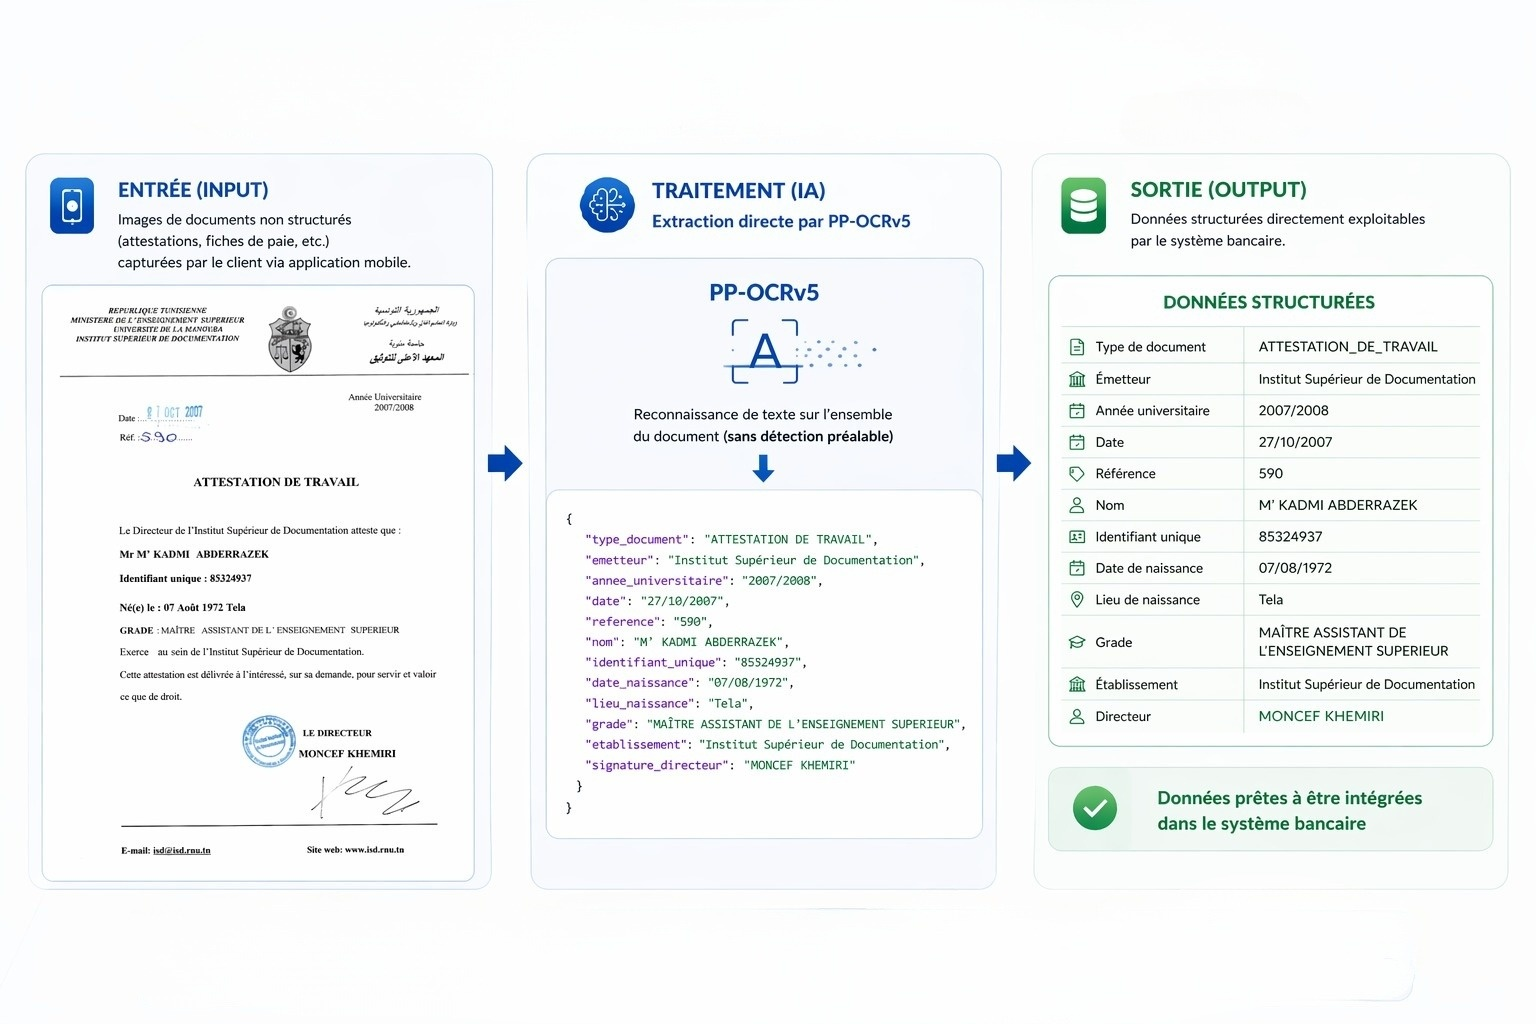
\includegraphics[width=0.75\textwidth]{images/image_ch3/pipline_1_phase.jpg}
  \caption{\textit{Pipeline CIN/Passeport}}
  \label{fig:ch3-pipeline-ia_cin-passeport}
\end{figure}

\textbf{Documents structurés (CIN, Passeport) :} une étape de détection d'objets (YOLO11m) précède l'extraction OCR. Cette approche en deux temps est nécessaire pour isoler avec précision les zones d'intérêt (données biométriques, numéro de série) sur des supports à géométrie variable.

\begin{figure}[H]
  \centering
  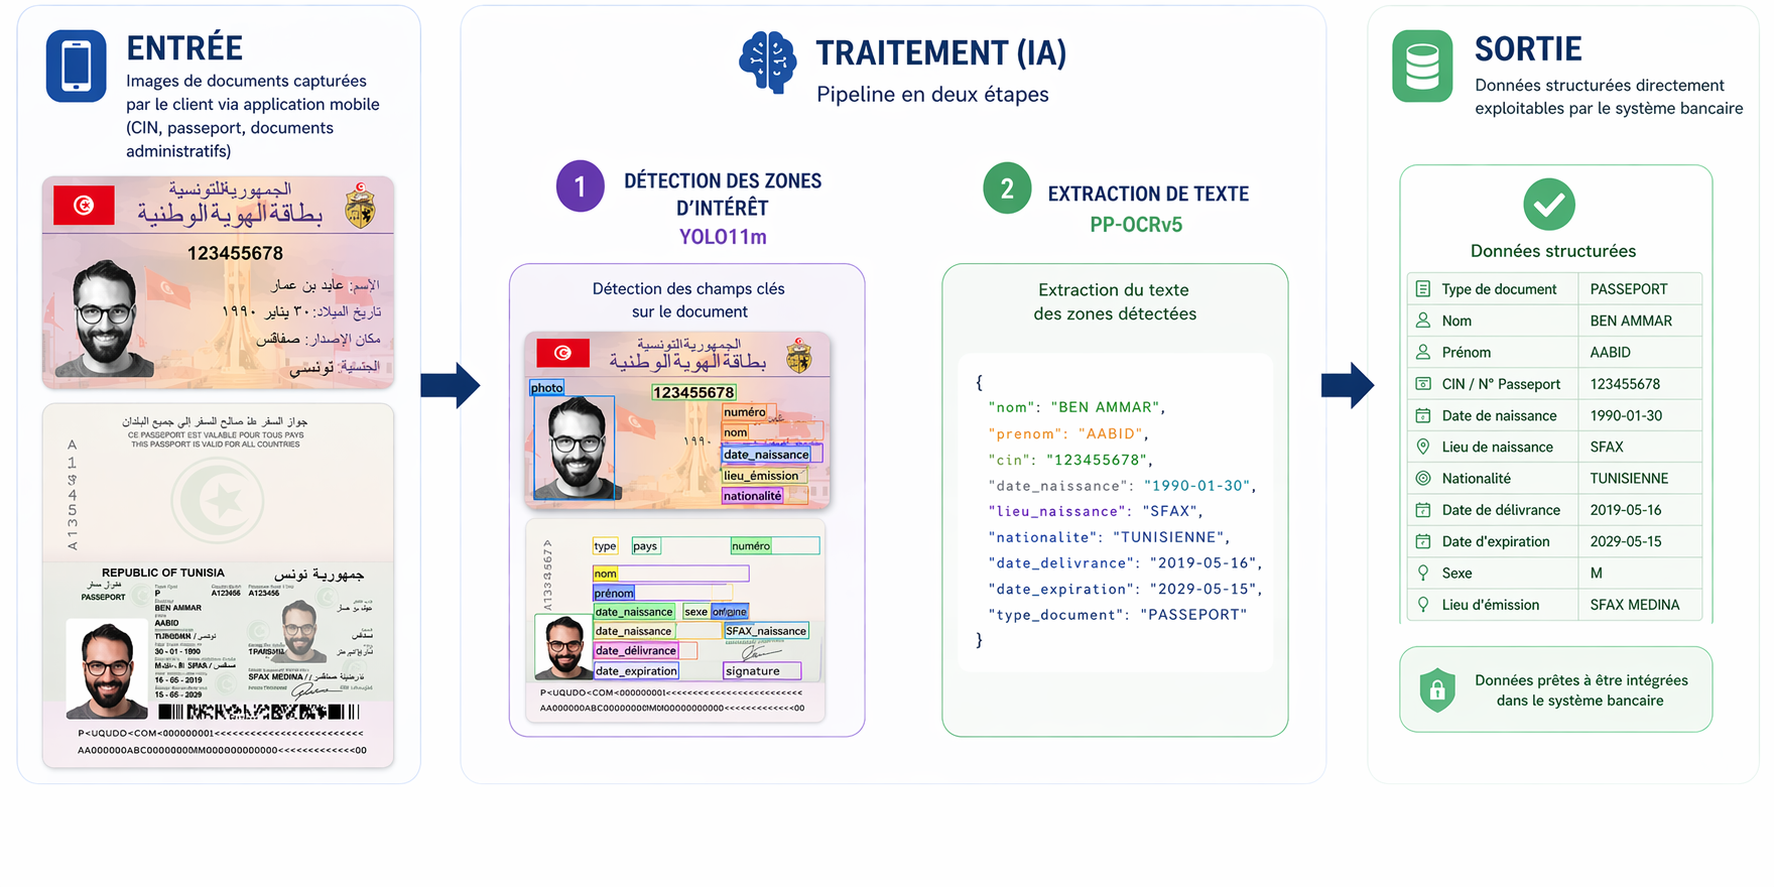
\includegraphics[width=0.75\textwidth]{images/image_ch3/pipline_2_phase.png}
  \caption{\textit{Pipeline autres documents}}
  \label{fig:ch3-pipeline-ia_autres-docs}
\end{figure}

\textbf{Documents non structurés (attestations, fiches de paie) :} l'extraction est réalisée directement par PP-OCRv5, sans étape de détection préalable. Cette rationalisation réduit sensiblement le temps d'inférence tout en maintenant une précision élevée sur des formats standardisés.

\subsection{Analyse des besoins documentaires}
\label{subsec:besoins-documentaires}

Chaque service bancaire implique un ensemble spécifique de documents à vérifier. Le tableau ci-dessous synthétise ces exigences et le pipeline IA correspondant.

\begin{table}[H]
  \centering
  \tiny
  \begin{tabular}{|l|l|l|}
    \toprule
    \rowcolor{bleu_principal}
    \textcolor{white}{\textbf{Service Métier}} & \textcolor{white}{\textbf{Documents Requis}} & \textcolor{white}{\textbf{Pipeline IA}} \\
    \midrule
    Ouverture de compte & CIN (recto/verso) ou Passeport & YOLO11m + PP-OCRv5 \\
    \midrule
    \rowcolor{gris_leger}
    Demande de crédit & CIN + Attestation de travail + Fiche de paie & YOLO11m + PP-OCRv5 (CIN) / PP-OCRv5 (docs fin.) \\
    \midrule
    Carte bancaire / Chéquier & Aucun document supplémentaire & Réutilisation données KYC \\
    \bottomrule
  \end{tabular}
  \caption{Matrice des documents requis par service et pipeline IA associé}
  \label{tab:ch3-besoins-doc}
\end{table}

Il convient de noter que le service carte bancaire et chéquier ne requiert aucune vérification documentaire supplémentaire : il s'appuie exclusivement sur le profil KYC déjà validé lors de l'ouverture de compte, ce qui allège le processus tout en garantissant la cohérence des données.

Cette cartographie des besoins documentaires oriente directement la stratégie de collecte et de constitution du dataset, présentée dans la section suivante.

\subsection{Collecte et composition du dataset}
\label{subsec:collecte-dataset}

La fiabilité d'une solution KYC bancaire ne repose pas sur la quantité brute de données, mais sur leur capacité à simuler l'imprévisibilité des conditions réelles : faible luminosité, arrière-plans complexes, captures mobiles en conditions non contrôlées. C'est sur ce principe qu'a été définie la stratégie de collecte.

\subsubsection*{Stratégie de collecte hybride}

Afin de construire un dataset à la fois structuré et robuste, deux canaux de collecte complémentaires ont été exploités :

\begin{itemize}
  \item \textbf{Open Source (Roboflow Universe) :} extraction de jeux de données préexistants comprenant des passeports internationaux et des échantillons de CIN tunisiennes, capturés en conditions idéales.

  \item \textbf{Données réelles (réseaux sociaux) :} collecte d'images de documents publiées en ligne (notamment des CIN déclarées perdues), présentant du bruit, des contre-jours et des masquages de confidentialité --- contraintes critiques reproduisant l'usage réel de l'application mobile.
\end{itemize}

\begin{table}[H]
  \centering
  \tiny
  \begin{tabular}{|l|p{3.5cm}|p{3.5cm}|p{3.5cm}|}
    \toprule
    \rowcolor{bleu_principal}
    \textcolor{white}{\textbf{Source}} & \textcolor{white}{\textbf{Avantage}} & \textcolor{white}{\textbf{Limite}} & \textcolor{white}{\textbf{Rôle}} \\
    \midrule
    Open Source (Roboflow) & Données propres, pré-annotées & Faible bruit --- peu réaliste & Pré-entraînement \\
    \midrule
    \rowcolor{gris_leger}
    Données réelles (réseaux sociaux) & Conditions réelles : bruit, contre-jour & Masquages agressifs & Robustesse \\
    \bottomrule
  \end{tabular}
  \caption{Analyse comparative des sources de données}
  \label{tab:ch3-sources-data}
\end{table}

La combinaison des deux sources compense leurs limites respectives --- l'open source apporte la structure, les données réelles apportent la robustesse face à l'imprévisibilité du terrain.

\subsubsection*{Distribution des classes}

Le dataset final totalise 685 instances, réparties de manière équilibrée entre les quatre classes d'intérêt :

\begin{table}[H]
  \centering
  \begin{tabular}{|l|c|c|l|}
    \toprule
    \rowcolor{bleu_principal}
    \textcolor{white}{\textbf{Classe}} & \textcolor{white}{\textbf{Instances}} & \textcolor{white}{\textbf{Proportion}} & \textcolor{white}{\textbf{Type de Traitement}} \\
    \midrule
    cinRecto & 200 & 29,2\% & YOLO11m + PP-OCRv5 \\
    \midrule
    \rowcolor{gris_leger}
    cinVerso & 202 & 29,5\% & YOLO11m + PP-OCRv5 \\
    \midrule
    passeport & 152 & 22,2\% & YOLO11m + PP-OCRv5 \\
    \midrule
    \rowcolor{gris_leger}
    Autre & 131 & 19,1\% & PP-OCRv5 (direct) \\
    \midrule
    \textbf{Total} & \textbf{685} & \textbf{100\%} & Hybride \\
    \bottomrule
  \end{tabular}
  \caption{Distribution du dataset par classe (source : Roboflow)}
  \label{tab:ch3-distribution-classes}
\end{table}

La quasi-parité entre cinRecto (200) et cinVerso (202) réflète une attention particulière à la couverture des deux faces de la CIN tunisienne, les deux étant requises lors de l'ouverture de compte. La classe Autre (131 instances) regroupe des captures partielles, des documents dégradés ou des images non identifiables --- utiles pour renforcer la robustesse du modèle face aux cas limites.

Si le sourcing réel apporte le réalisme nécessaire, il introduit un obstacle majeur : les données sont inexploitables en l'état à cause des masquages. Cela rend la phase suivante de Data Engineering (Restauration) non seulement utile, mais indispensable pour créer une vérité terrain supervisée.


%=============================================================
\section{Préparation des données (ingénierie des données)}
\label{sec:data-preparation}
%=============================================================

Les données collectées sur les réseaux sociaux, bien que cruciales pour le réalisme, posent un défi majeur de supervision : les masques de confidentialité --- traits de feutre, bandes noires, flous numériques --- empêchent YOLO d'apprendre la structure complète et les points d'ancrage réels des documents. Pour transformer ces données inexploitables en une vérité terrain (Ground Truth) de haute précision, deux stratégies complémentaires ont été déployées, adaptées à la complexité de chaque face du document.

\subsection{Restauration et génération de données}
\label{subsec:restauration-generation}

\subsubsection*{CIN recto --- restauration par Deep Inpainting}

Pour le recto, l'enjeu était double : conserver l'authenticité visuelle de la photo d'identité et du fond, tout en rendant le numéro de carte exploitable par l'OCR. Le processus se déroule en trois phases :

\begin{itemize}
  \item \textbf{Nettoyage localisé :} application d'algorithmes de Deep Inpainting (via ObjectRemover) sur la zone du numéro masqué. L'IA reconstruit les motifs de sécurité (guillochis) en analysant les pixels environnants.

  \item \textbf{Réinjection typographique :} superposition d'un numéro de remplacement dans la police OCR-B (norme ISO) via Figma, garantissant alignement et espacement identiques aux documents officiels.

  \item \textbf{Réalisme contextuel :} chaque insertion respecte la signature optique d'origine par Blur Matching (flou gaussien calibré sur le grain du capteur) et Glare Integration (fusion avec les zones de surexposition), éliminant toute « anomalie de perfection » qui trahirait l'origine synthétique de la donnée.
\end{itemize}

\begin{figure}[H]
  \centering
  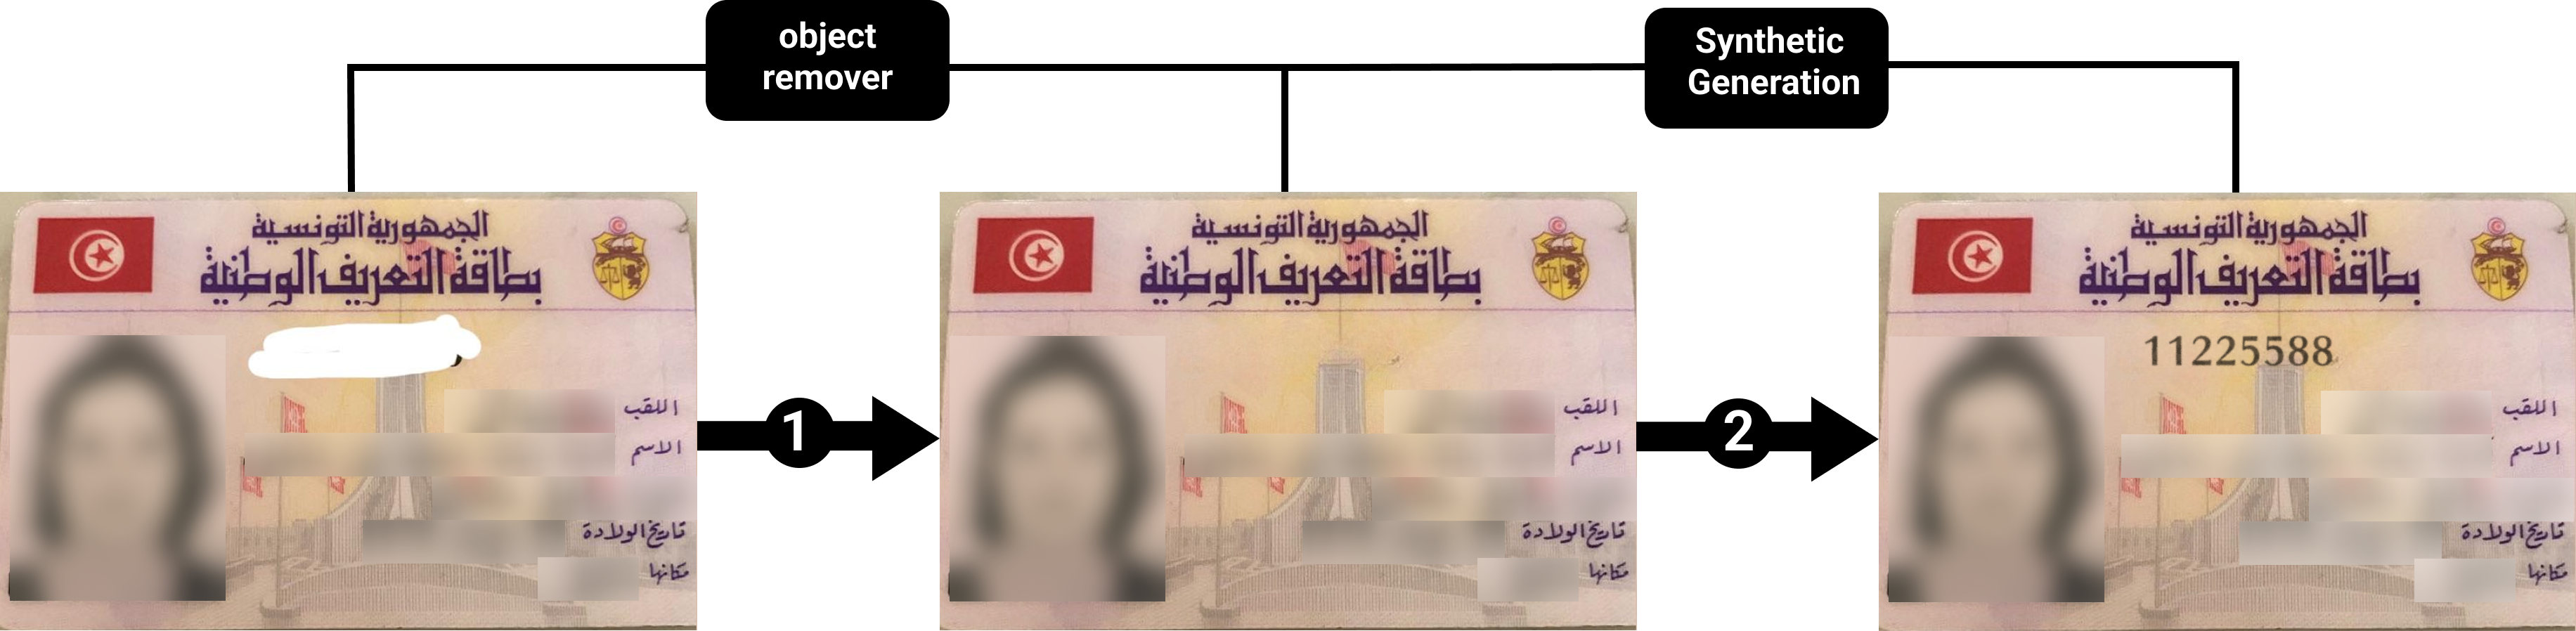
\includegraphics[width=0.75\textwidth]{images/image_ch3/Processus de_restauration_CIN Recto.png}
  \caption{\textit{Figure 3.1 --- Processus de restauration CIN Recto}}
  \label{fig:ch3-restauration-recto}
\end{figure}

\begin{figure}[H]
  \centering
  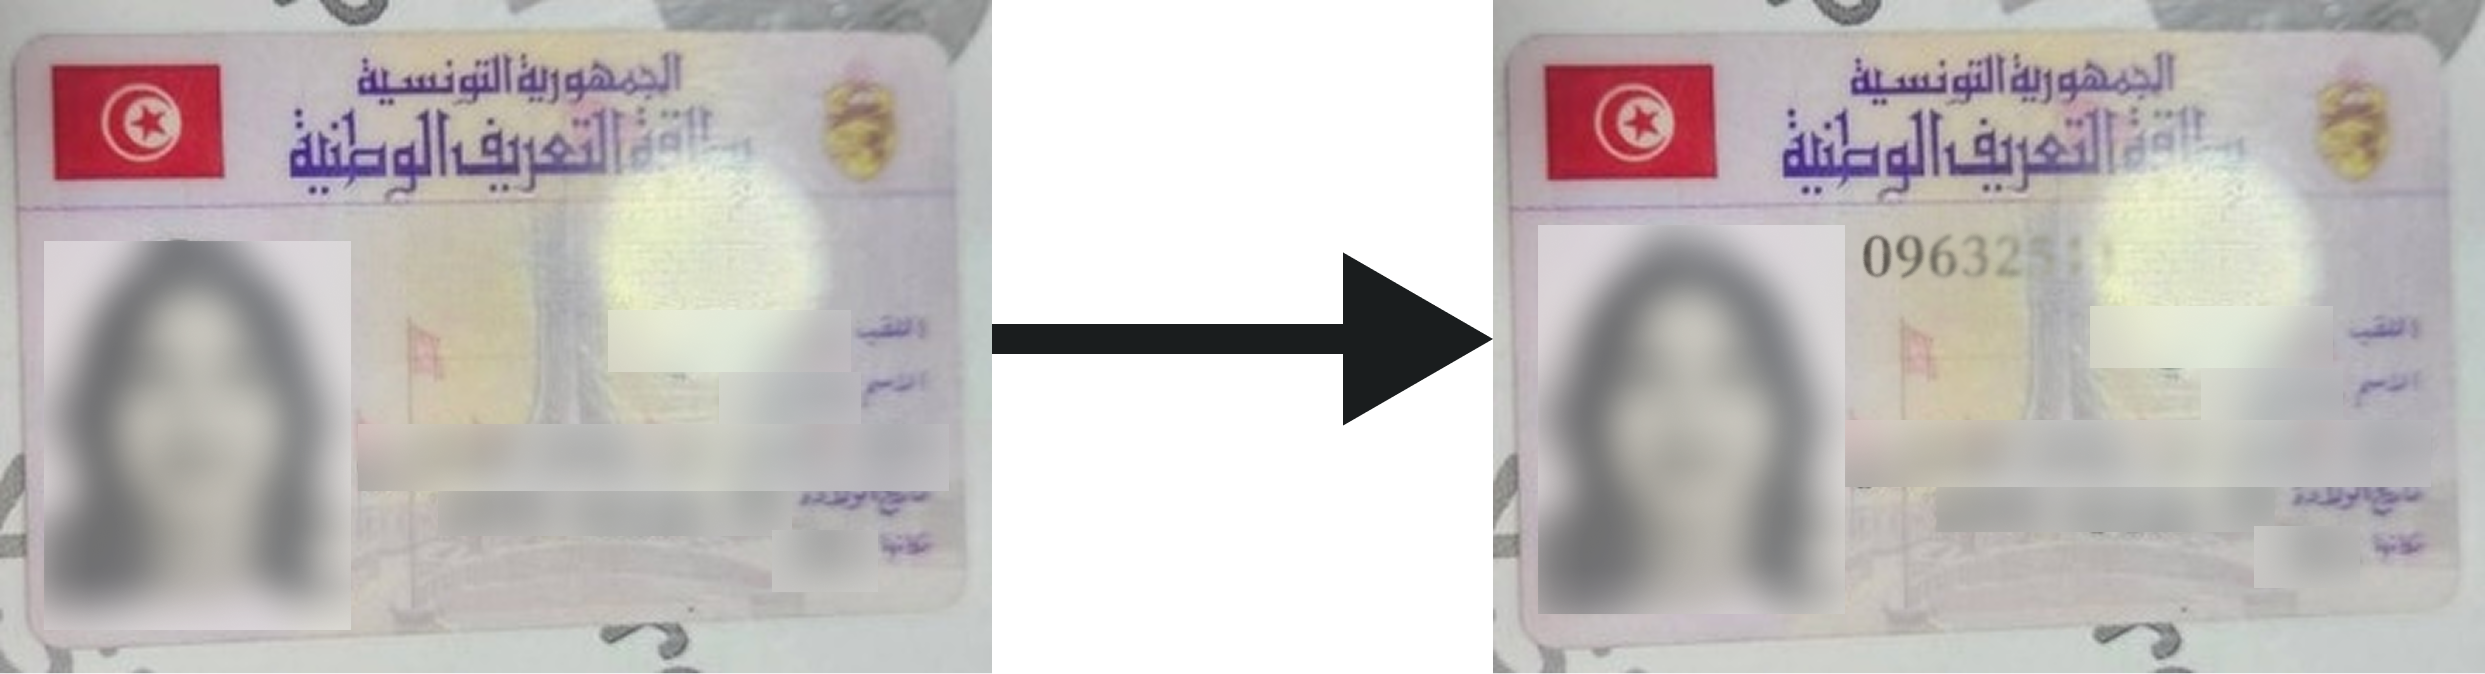
\includegraphics[width=0.75\textwidth]{images/image_ch3/Simulation_de_contraintes_optiques réelles.png}
  \caption{\textit{Figure 3.2 --- Simulation de contraintes optiques réelles}}
  \label{fig:ch3-contraintes-optiques}
\end{figure}

\subsubsection*{CIN verso --- génération automatisée par Data Factory Python}

Le verso, dont la densité textuelle est plus élevée, nécessitait une approche différente. Plutôt que de traiter chaque image individuellement, nous avons créé une matrice de génération à partir d'un document authentique :

\begin{itemize}
  \item \textbf{Génération du template de base :} plutôt que de dessiner un fond artificiel, nous avons pris une image de CIN réelle dont nous avons intégralement effacé les mentions textuelles via ObjectRemover. Le résultat est un template nu qui conserve la texture physique authentique --- grain numérique, ombres portées, irrégularités d'éclairage --- d'un document téléversé par mobile.

  \item \textbf{Data Factory Python :} un script automatise le remplissage des champs (Nom, Prénom du père, Mère, Adresse) en générant des identités aléatoires positionnées avec précision sur le template. Cette méthode produit des centaines de variantes parfaitement étiquetées sur un support qui « trompe » l'œil du modèle en lui faisant croire qu'il traite un document 100\% réel.
\end{itemize}

\begin{figure}[H]
  \centering
  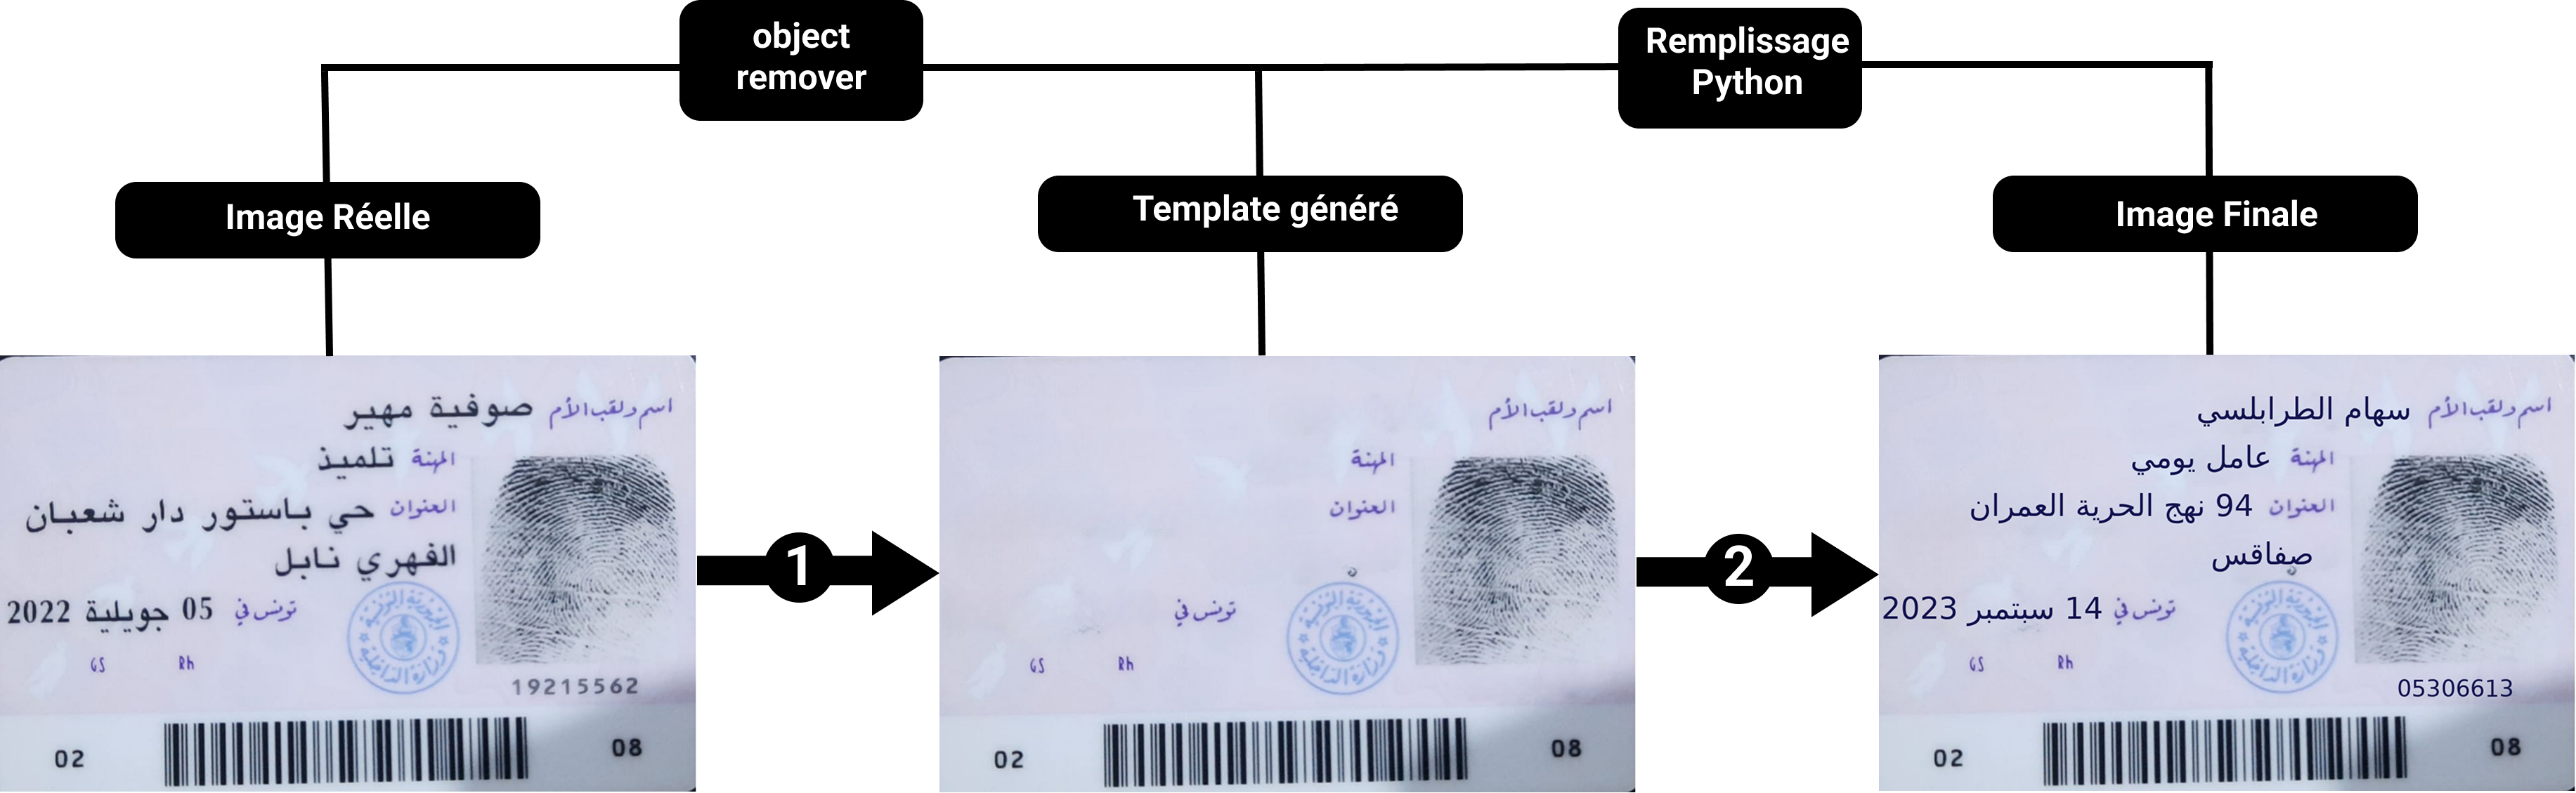
\includegraphics[width=0.75\textwidth]{images/image_ch3/Pipeline_creation_template_verso.png}
  \caption{\textit{Figure 3.3 --- Pipeline de création du template Verso}}
  \label{fig:ch3-template-verso}
\end{figure}

Une fois ce dataset restauré et enrichi, il convient de lui donner un sens mathématique pour l'IA. La phase de labellisation intervient alors pour définir précisément les zones d'intérêt, transformant les images brutes en données d'apprentissage supervisé.

\subsection{Labellisation : construction de la vérité terrain}
\label{subsec:labellisation}

Une fois le dataset restauré, il convient de lui donner un sens mathématique pour l'IA. La labellisation consiste à définir des Bounding Boxes autour de chaque champ critique, transformant les images brutes en données d'apprentissage supervisé.

\subsubsection*{Ontologie des classes}

Trois ontologies distinctes ont été définies selon le type de document :

\begin{itemize}
  \item \textbf{CIN Recto :} address, cin, dob, first\_name, flag1, flag2, full\_name, header\_text, image, last\_name, num\_cin, pob.

  \item \textbf{CIN Verso :} address, barcode, finger\_print, flag3, issue\_date, mother\_name, print\_id, profession.

  \item \textbf{Passeport :} address, dob, first\_name, image, last\_name, num\_cin, pob, num\_pass.
\end{itemize}

\subsubsection*{Méthodologie hybride : du Gold Standard à l'Auto-Labeling}

Face au volume de données à annoter, une approche hybride en trois phases a été adoptée pour concilier efficacité et précision :

\begin{enumerate}
  \item \textbf{Amorçage manuel (Gold Standard) :} labellisation manuelle des 50 premières images de chaque catégorie sur Roboflow, constituant un jeu de référence de haute précision.

  \item \textbf{Auto-labeling assisté :} un modèle YOLO pré-entraîné sur ces 50 images suggère automatiquement les boîtes sur les images restantes, réduisant considérablement le temps d'annotation.

  \item \textbf{Vérification humaine systématique :} chaque boîte suggérée est ajustée manuellement pour que ses bords touchent exactement les caractères --- condition critique pour la qualité de l'extraction OCR.
\end{enumerate}

\subsubsection*{Contrainte des Tight Bounding Boxes}

Une règle stricte a été appliquée : la boîte doit englober le texte au pixel près sans inclure de bruit environnant. Une boîte trop large incorpore des éléments décoratifs qui perturbent l'OCR ; une boîte trop serrée coupe les jambages de certains caractères (tels que 'p' ou 'q'), dégradant la précision de la reconnaissance. Cette rigueur constitue la condition sine qua non d'une extraction OCR performante.

\begin{figure}[H]
  \centering
  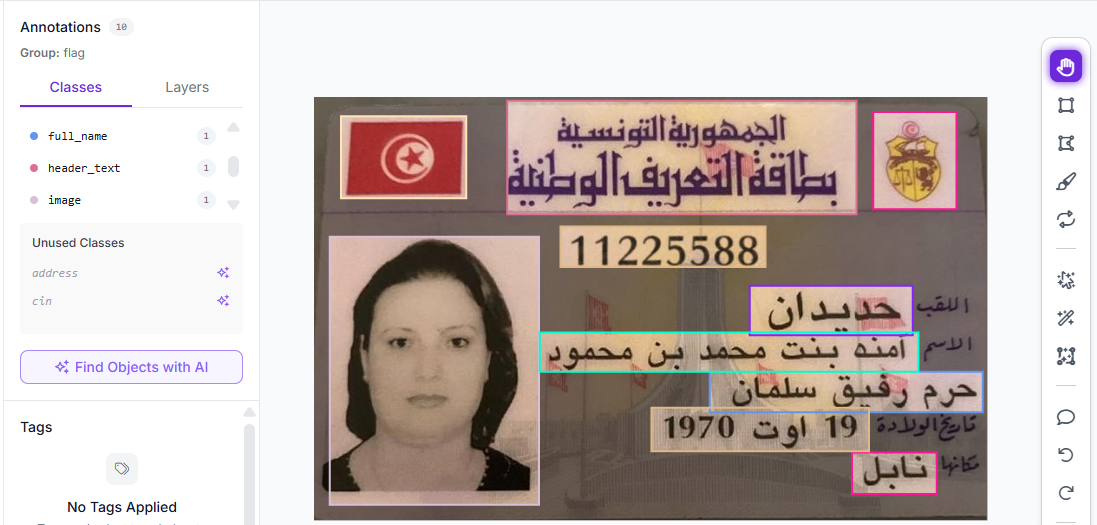
\includegraphics[width=0.75\textwidth]{images/image_ch3/roboflow.png}
  \caption{\textit{Interface Roboflow illustrant la précision des Tight Bounding Boxes sur une CIN}}
  \label{fig:ch3-bounding-boxes}
\end{figure}

Le dataset ainsi labellisé constitue une base d'apprentissage rigoureuse. Cependant, 685 instances restent insuffisantes pour garantir la robustesse du modèle face aux aléas d'une capture mobile réelle. La phase d'augmentation contrôlée répond à ce défi.

\subsection{Augmentation contrôlée : simulation de la variabilité réelle}
\label{subsec:augmentation}

Plutôt qu'une augmentation aléatoire, nous avons appliqué une stratégie différenciée selon la complexité de chaque tâche pour éviter le surapprentissage via la plateforme Roboflow, simulant les contraintes physiques du monde réel tout en évitant le surapprentissage.

\subsubsection*{Coefficients d'augmentation différenciés}

Le volume final a été calibré pour éviter le surapprentissage tout en assurant une couverture représentative des scénarios réels :

\begin{table}[H]
  \centering
  \begin{tabular}{|l|c|c|c|l|}
    \toprule
    \rowcolor{bleu_principal}
    \textcolor{white}{\textbf{Pipeline}} & \textcolor{white}{\textbf{Source}} & \textcolor{white}{\textbf{Coefficient}} & \textcolor{white}{\textbf{Total}} & \textcolor{white}{\textbf{Focus}} \\
    \midrule
    Classification Globale & 473 & ×10 & 4\,730 & Invariance contextuelle globale \\
    \midrule
    \rowcolor{gris_leger}
    CIN Recto & 712 & ×4 & 2\,884 & Perspective et alignement YOLO \\
    \midrule
    CIN Verso & 182 & ×4 & 728 & Précision OCR et netteté \\
    \midrule
    \rowcolor{gris_leger}
    Passeport & 158 & ×4 & 644 & Précision OCR et netteté \\
    \bottomrule
  \end{tabular}
  \caption{Coefficients d'augmentation par pipeline et volumes finaux obtenus}
  \label{tab:ch3-augmentation-coeff}
\end{table}

\subsubsection*{Paramètres d'augmentation et impacts visuels}

Trois axes de transformation ont été retenus, chacun répondant à une contrainte physique identifiée :

\paragraph{A. Invariance spatiale (géométrie \& perspective)}

Ces transformations compensent les erreurs de manipulation humaine. Un utilisateur ne tient jamais son smartphone parfaitement parallèle au document, ce qui crée des distorsions géométriques.

\begin{figure}[H]
  \centering
  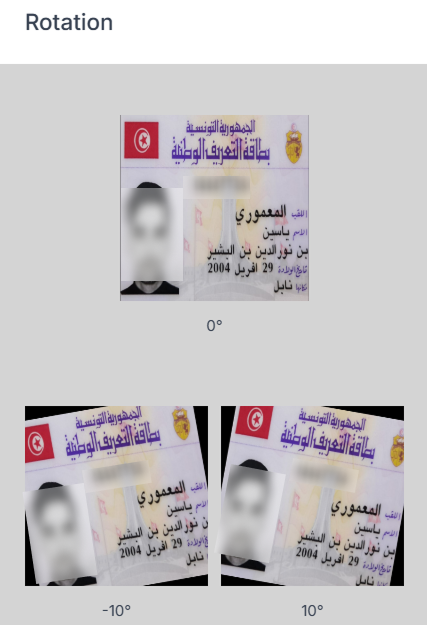
\includegraphics[width=0.75\textwidth]{images/image_ch3/rotation.png}
  \caption{\textit{Illustration de l'augmentation par rotation ($-$10°, 0°, +10°)}}
  \label{fig:ch3-rotation}
\end{figure}

\begin{itemize}
  \item \textbf{Rotation :} indispensable pour que YOLO détecte la carte même si elle est présentée de travers.
\end{itemize}

\paragraph{B. Invariance photométrique (lumière \& couleur)}

L'objectif est de rendre l'extraction d'information indépendante de l'éclairage ambiant ou de la qualité du capteur.

\begin{figure}[H]
  \centering
  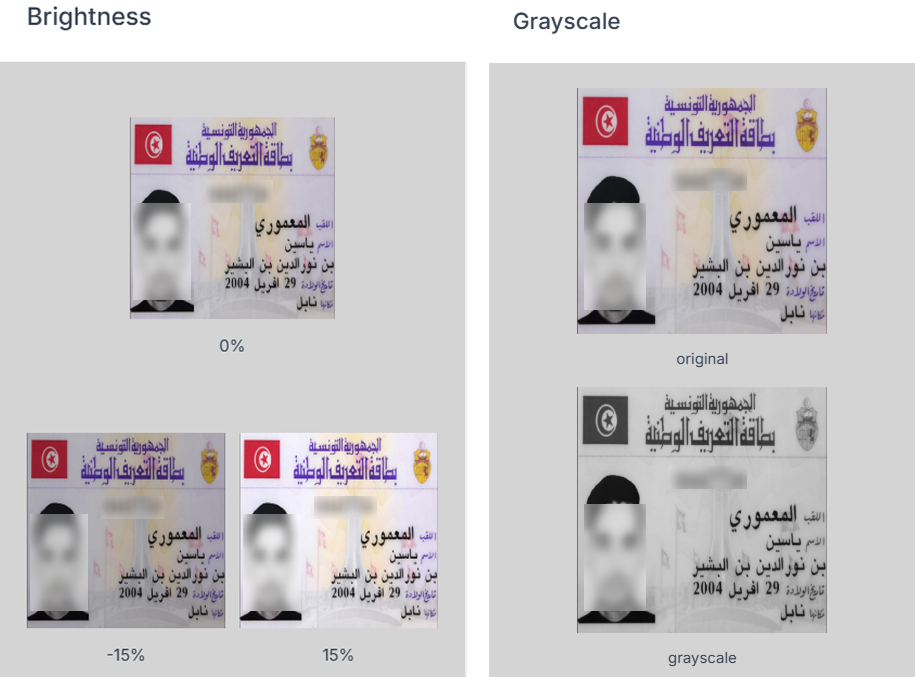
\includegraphics[width=0.75\textwidth]{images/image_ch3/lumino_grayscale.png}
  \caption{\textit{Illustration de l'augmentation photométrique : variations de luminosité et niveaux de gris}}
  \label{fig:ch3-photometrie}
\end{figure}

\begin{itemize}
  \item \textbf{Luminosité :} reproduit les variations entre une pièce sombre et un éclairage direct (éblouissement par le flash).

  \item \textbf{Grayscale :} habitue le modèle à reconnaître la structure de la CIN même sur des captures en noir et blanc ou des photocopies de faible qualité.
\end{itemize}

\paragraph{C. Résilience optique (flou \& bruit capteur)}

\begin{figure}[H]
  \centering
  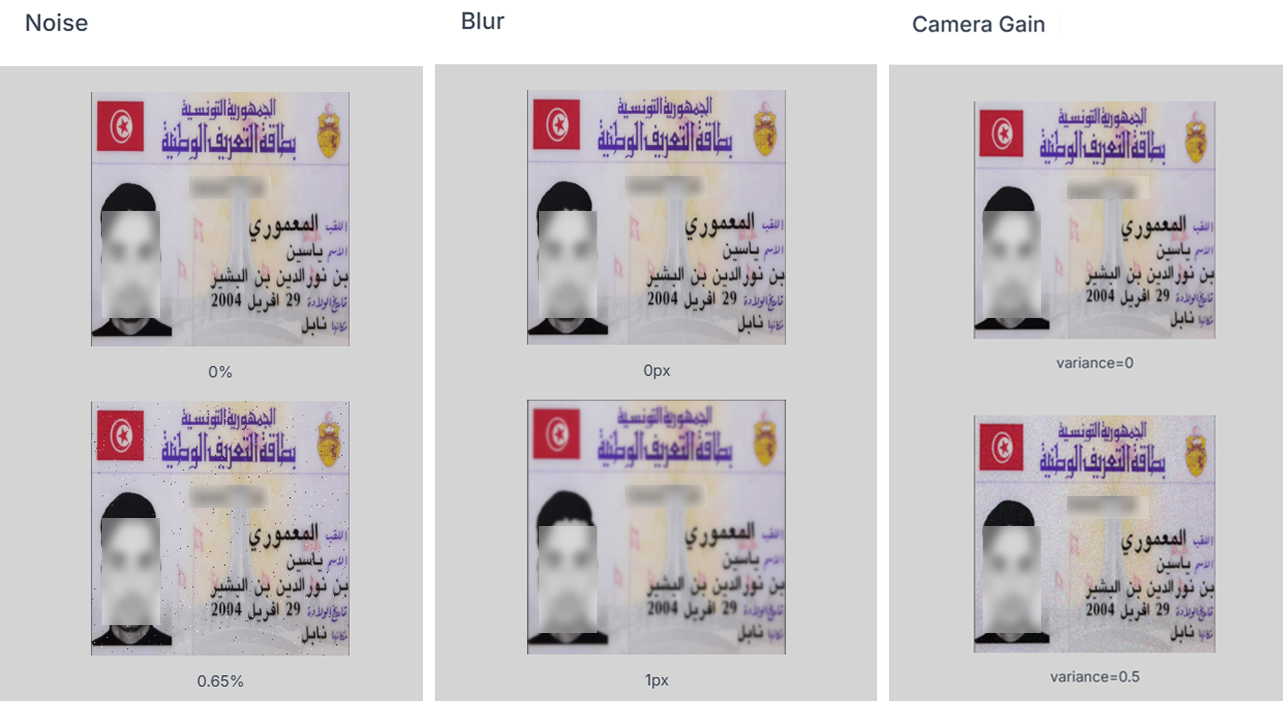
\includegraphics[width=0.75\textwidth]{images/image_ch3/bruit_flou_gainCamera.png}
  \caption{\textit{Illustration de la résilience optique : bruit, flou et gain de caméra}}
  \label{fig:ch3-resilience-optique}
\end{figure}

\begin{itemize}
  \item \textbf{Bruit :} ajout de grain pour simuler les capteurs de smartphones d'entrée de gamme en basse lumière.

  \item \textbf{Gain de caméra :} simule l'amplification ISO pour la robustesse à l'exposition.

  \item \textbf{Flou :} modélise les imprécisions de mise au point pour forcer l'extraction de traits robustes.
\end{itemize}

\subsubsection*{Configurations Roboflow par pipeline}

\begin{table}[H]
  \centering
  \small
  \begin{tabular}{|l|c|c|c|c|}
    \toprule
    \rowcolor{bleu_principal}
    \textcolor{white}{\textbf{Paramètre}} & \textcolor{white}{\textbf{Classification}} & \textcolor{white}{\textbf{CIN Recto}} & \textcolor{white}{\textbf{CIN Verso}} & \textcolor{white}{\textbf{Passeport}} \\
    \midrule
    Sorties / exemple & 3 & 4 & 4 & 4 \\
    \midrule
    \rowcolor{gris_leger}
    Rotation & ±10° & ±10° & ±10° & ±5° \\
    \midrule
    Niveaux de gris & --- & 5\% images & 5\% images & --- \\
    \midrule
    \rowcolor{gris_leger}
    Luminosité & ±25\% & ±10\% & ±10\% & ±15\% \\
    \midrule
    Flou simple & $\leq$1 px & $\leq$0,5 px & $\leq$0,5 px & $\leq$0,4 px \\
    \midrule
    \rowcolor{gris_leger}
    Bruit & $\leq$0,69\% & $\leq$0,3\% & $\leq$0,3\% & $\leq$0,3\% \\
    \midrule
    Gain de caméra & --- & 0,06\% & 0,06\% & --- \\
    \midrule
    \rowcolor{gris_leger}
    \textbf{Total dataset} & \textbf{4\,932} & \textbf{3\,004} & \textbf{806} & \textbf{709} \\
    \bottomrule
  \end{tabular}
  \caption{Configurations Roboflow par pipeline}
  \label{tab:ch3-roboflow-config}
\end{table}

Cette stratégie d'augmentation a pour objectif d'enrichir notre base d'entraînement avec un volume de données diversifié, permettant ainsi au modèle d'affiner ses capacités d'apprentissage et d'améliorer sa précision globale.

Le dataset ainsi constitué --- restauré, labellisé et augmenté --- offre une base d'entraînement solide. La section suivante détaille l'architecture du pipeline IA retenu et les paramètres d'entraînement associés.


%=============================================================
\section{Modélisation}
\label{sec:modelisation}
%=============================================================

Le dataset ainsi constitué --- restauré, labellisé et augmenté --- constitue le socle sur lequel reposent les décisions de modélisation. Cette section décrit l'architecture du pipeline IA retenu et les paramètres d'entraînement pour chacun des modèles développés.

%-------------------------------------------------------------
\subsection{Architecture globale du système IA}
\label{subsec:architecture-ia}
%-------------------------------------------------------------

Le système IA est structuré en deux pipelines distincts selon la nature du document traité (voir Figure~\ref{fig:ch3-pipeline-ia_cin-passeport} et Figure~\ref{fig:ch3-pipeline-ia_autres-docs}, section 3.1.1). Pour les documents structurés --- CIN et passeport --- le pipeline enchaîne quatre services indépendants exposés chacun via une API REST FastAPI :

\begin{enumerate}
  \item \textbf{Service de classification} (port 8005) : reçoit l'image capturée et identifie le type de document parmi cinq classes (\texttt{CIN\_RECTO}, \texttt{CIN\_VERSO}, \texttt{PASSPORT}, \texttt{ATTESTATION\_TRAVAIL}, \texttt{FICHE\_PAIE}) grâce à un modèle YOLOcls.
  \item \textbf{Service de capture} (ports 8001/8006) : détecte la présence du document dans le flux vidéo en temps réel via YOLOv8n et déclenche la capture automatique dès stabilisation.
  \item \textbf{Service OCR} (port 8002) : localise les champs par YOLOv11m, recadre chaque zone et en extrait le texte via PaddleOCR PP-OCRv5.
  \item \textbf{Service de comparaison faciale} (port 8007) : capture le selfie et compare la photo extraite du document avec le visage de l'utilisateur.
\end{enumerate}

Ce découplage en microservices garantit qu'une mise à jour d'un modèle n'impacte aucun autre service, conformément aux exigences de maintenabilité définies en section 4.3.

%-------------------------------------------------------------
\subsection{Détection de présence du document --- YOLOv8n}
\label{subsec:yolov8n-presence}
%-------------------------------------------------------------

Avant toute extraction, le système doit s'assurer que le document est correctement cadré et de qualité suffisante. Ce rôle est assuré par trois services de capture exploitant chacun un modèle YOLOv8n léger, adapté à une inférence en temps réel sur flux vidéo :

\begin{itemize}
  \item \texttt{capture-cin} (port 8001) : CIN recto et verso.
  \item \texttt{capture-passport} (port 8006) : passeport.
  \item \texttt{capture-face} (port 8007) : selfie biométrique.
\end{itemize}

\noindent\textbf{Paramètres de détection.} Chaque frame est analysée à 640 $\times$ 640 pixels avec :

\begin{itemize}
  \item Seuil de détection : 0,25 (sensibilité maximale).
  \item Seuil de validation métier : 0,50 (décision de capture).
  \item Stabilisation : 5 frames consécutives valides requises avant déclenchement, éliminant les fausses confirmations dues aux mouvements brusques.
  \item Stockage : image recadrée et agrandie, enregistrée dans MinIO à 97\,\% de qualité JPEG pour préserver la lisibilité OCR en aval.
\end{itemize}

\noindent\textbf{États retournés au frontend.} Le service communique trois états en temps réel guidant l'utilisateur sans action manuelle :

\begin{itemize}
  \item \texttt{ABSENT} : aucun document détecté dans le cadre.
  \item \texttt{DETECTED} : document présent mais pas encore stabilisé.
  \item \texttt{CONFIRMED} : capture validée, transmission au pipeline OCR.
\end{itemize}

Ce service constitue le verrou qualité d'entrée du pipeline.

%-------------------------------------------------------------
\subsection{Détection des champs texte --- YOLOv11m}
\label{subsec:yolov11m-champs}
%-------------------------------------------------------------

Comme établi au chapitre 2, YOLOv11m a été retenu pour sa supériorité en précision de localisation sur des objets de petite taille dans des images à haute résolution. Il intervient ici non pour détecter des objets génériques, mais pour localiser avec précision chaque champ textuel sur un document d'identité.

\subsubsection*{Stratégie : trois modèles spécialisés}

La décision de former trois modèles distincts --- un par type de document --- répond à une contrainte fondamentale : les ontologies de classes sont incompatibles entre documents.

\begin{itemize}
  \item \textbf{CIN Recto} : 12 classes incluant \texttt{last\_name}, \texttt{first\_name}, \texttt{full\_name}, \texttt{num\_cin}, \texttt{dob}, \texttt{pob}, \texttt{image}, \texttt{header\_text}, \texttt{flag1}, \texttt{flag2}. La disposition est arabe de droite à gauche, avec des zones de texte compactes.
  \item \textbf{CIN Verso} : 8 classes dont \texttt{mother\_name}, \texttt{profession}, \texttt{address}, \texttt{issue\_date}, \texttt{print\_id}, \texttt{barcode}, \texttt{finger\_print}, \texttt{flag3}. Le champ adresse est multi-lignes et occupe une surface importante.
  \item \textbf{Passeport} : champs bilingues arabe/latin, \texttt{last\_name}, \texttt{first\_name}, \texttt{num\_pass}, \texttt{num\_cin}, \texttt{dob}, \texttt{pob}, \texttt{image}, \texttt{address}. Format portrait ($3$:$4$), densité textuelle plus forte.
\end{itemize}

Un modèle unique entraîné sur les trois documents produirait des ambiguïtés de classes (un champ \texttt{dob} sur la CIN et un champ \texttt{dob} sur le passeport n'ont pas le même format ni la même position) et dégraderait la précision des bounding boxes.

\subsubsection*{Paramètres d'entraînement}

Les trois modèles partagent la même architecture de base YOLOv11m pré-entraînée sur COCO, avec un \textit{fine-tuning} par transfert d'apprentissage. Le Tableau~\ref{tab:ch3-params-yolo} présente les paramètres comparatifs.

\small
\begin{longtable}{|l|c|c|c|}
  \rowcolor{bleu_principal}
  \textcolor{white}{\textbf{Paramètre}} & \textcolor{white}{\textbf{CIN Recto}} & \textcolor{white}{\textbf{CIN Verso}} & \textcolor{white}{\textbf{Passeport}} \\
  \endfirsthead
  \rowcolor{bleu_principal}
  \textcolor{white}{\textbf{Paramètre}} & \textcolor{white}{\textbf{CIN Recto}} & \textcolor{white}{\textbf{CIN Verso}} & \textcolor{white}{\textbf{Passeport}} \\
  \endhead
  \midrule
  Images originales & 712 & 532 & 488 \\
  \midrule
  \rowcolor{gris_leger}
  Coefficient augmentation & $\times$4 & $\times$4 & $\times$3 \\
  \midrule
  Images entraînement & 2\,848 & 2\,128 & 1\,464 \\
  \midrule
  \rowcolor{gris_leger}
  Images validation & 156 & 148 & 137 \\
  \midrule
  Images test & 70 & 60 & 50 \\
  \midrule
  \rowcolor{gris_leger}
  Résolution & 1280 $\times$ 1280 px & 1280 $\times$ 1280 px & 1280 $\times$ 1280 px \\
  \midrule
  Batch size & 8 & 8 & 8 \\
  \midrule
  \rowcolor{gris_leger}
  Époques max & 150 & 150 & 150 \\
  \midrule
  Patience (early stop) & 40 & 40 & 40 \\
  \midrule
  \rowcolor{gris_leger}
  Optimiseur & AdamW & AdamW & AdamW \\
  \midrule
  Taux d'apprentissage $lr_0$ & 0,001 & 0,001 & 0,001 \\
  \midrule
  \rowcolor{gris_leger}
  $lr$ final ($lrf$) & 0,01 & 0,01 & 0,01 \\
  \midrule
  Weight decay & 0,0003 & 0,0003 & 0,0004 \\
  \midrule
  \rowcolor{gris_leger}
  Warmup époques & 3 & 3 & 3 \\
  \midrule
  Scheduler LR & Cosinus & Cosinus & Cosinus \\
  \midrule
  \rowcolor{gris_leger}
  Loss box & 7,5 & 7,5 & 7,5 \\
  \midrule
  Loss cls & 0,5 & 0,5 & 0,4 \\
  \midrule
  \rowcolor{gris_leger}
  Loss dfl & 1,5 & 1,5 & 1,5 \\
  \midrule
  Scale (augmentation) & 0,20 & 0,10 & 0,15 \\
  \midrule
  \rowcolor{gris_leger}
  Translate & 0,03 & 0,04 & 0,04 \\
  \midrule
  Degrees & 2,0° & 2,0° & 3,0° \\
  \midrule
  \rowcolor{gris_leger}
  Mosaic / Mixup / Flip & Désactivés & Désactivés & Désactivés \\
  \bottomrule
  \caption{Paramètres comparatifs d'entraînement des trois modèles YOLOv11m}
  \label{tab:ch3-params-yolo}
\end{longtable}
\normalsize

Plusieurs choix méritent d'être explicités :

\begin{itemize}
  \item \textbf{Résolution 1\,280 $\times$ 1\,280 px :} les champs texte comme \texttt{num\_cin} ou \texttt{dob} occupent moins de 80 pixels de hauteur sur un document photographié de face --- une résolution de 640 px les rendrait illisibles pour l'OCR en aval.
  \item \textbf{Weight decay passeport (0,0004) :} légèrement supérieur à celui de la CIN (0,0003) pour compenser un dataset plus réduit (1\,464 images contre 2\,848).
  \item \textbf{Scale verso réduit à 0,10 :} protège la zone MRZ (\textit{Machine Readable Zone}) en bas de carte, dont une déformation excessive casserait la structure de lecture.
  \item \textbf{Mosaic / Mixup / Flip désactivés :} un document retourné ou composite n'existe pas en production --- ces augmentations introduiraient des cas irréalistes.
\end{itemize}

\subsubsection*{Résultats d'entraînement}

% ── Bloc YOLO ────────────────────────────────────────────────
\begin{tcolorbox}[
  enhanced,
  breakable,
  colback    = yolo_bg,
  colframe   = yolo_border,
  arc        = 4pt,
  boxrule    = 1.2pt,
  drop shadow,
  attach boxed title to top left = {yshift=-3mm, xshift=8mm},
  boxed title style = {
    colback   = yolo_header,
    colframe  = yolo_border,
    arc       = 3pt,
    boxrule   = 0.8pt,
    fontupper = \bfseries\color{white}\small
  },
  title = {\faSearch\quad Métriques de détection d'objets --- YOLO}
]

\noindent Les performances du modèle YOLOv11m sont évaluées selon les métriques standard d'Ultralytics, adaptées ici à la détection de champs textuels sur documents d'identité.

\medskip
\noindent\textbf{Concepts fondamentaux.} Toute prédiction est classée en l'une des quatre catégories :

\smallskip
\begin{center}
\small
\begin{tabular}{>{\bfseries}l p{9cm}}
  \rowcolor{bleu_principal!12}
  Catégorie & Signification dans le contexte KYC \\[2pt]
  \midrule
  TP & Le modèle détecte un champ textuel qui existe réellement sur le document. \\[3pt]
  FP & Le modèle prédit un champ absent du document (fausse alarme). \\[3pt]
  FN & Le modèle rate un champ présent --- champ critique manqué. \\[3pt]
  TN & Aucune détection là où aucun champ n'est attendu. \\
\end{tabular}
\end{center}

\medskip
\noindent\textbf{Métriques dérivées.}

\medskip

% Précision
\noindent\textcolor{bleu_clair}{\ding{72}}\; \textcolor{bleu_clair}{\textbf{Précision (Precision) :}}

\noindent La précision mesure la fiabilité des détections : sur toutes les zones prédites comme champs, combien sont effectivement des champs réels ?

\begin{equation*}
  P = \frac{TP}{TP + FP}
\end{equation*}

\noindent où $TP$ est le nombre de vrais positifs et $FP$ le nombre de faux positifs. Une précision élevée signifie peu de faux cadres autour de zones sans texte.

\medskip

% Rappel
\noindent\textcolor{bleu_clair}{\ding{72}}\; \textcolor{bleu_clair}{\textbf{Rappel (Recall) :}}

\noindent Le rappel mesure le taux de couverture : sur tous les champs présents dans le document, combien le modèle en a-t-il détectés ?

\begin{equation*}
  R = \frac{TP}{TP + FN}
\end{equation*}

\noindent où $FN$ est le nombre de faux négatifs. Un rappel élevé garantit qu'aucun champ critique (\texttt{num\_cin}, \texttt{dob}) n'est omis.

\medskip

% F1
\noindent\textcolor{bleu_clair}{\ding{72}}\; \textcolor{bleu_clair}{\textbf{Score F1 :}}

\noindent Moyenne harmonique de la précision et du rappel, synthétisant les deux en un seul indicateur équilibré.

\begin{equation*}
  F_1 = \frac{2 \times P \times R}{P + R}
\end{equation*}

\medskip

% IoU
\noindent\textcolor{bleu_clair}{\ding{72}}\; \textcolor{bleu_clair}{\textbf{IoU (\textit{Intersection over Union}) :}}

\noindent Mesure la précision spatiale de la boîte prédite en calculant le chevauchement entre la boîte prédite $\hat{B}$ et la vérité terrain $B$.

\begin{equation*}
  \text{IoU} = \frac{\text{Aire}(\hat{B} \cap B)}{\text{Aire}(\hat{B} \cup B)}
\end{equation*}

\noindent Un score de 1 indique une superposition parfaite — condition indispensable pour que le crop transmis à PaddleOCR soit exploitable.

\medskip

% mAP50
\noindent\textcolor{bleu_clair}{\ding{72}}\; \textcolor{bleu_clair}{\textbf{mAP50 :}}

\noindent Précision moyenne (\textit{mean Average Precision}) calculée à un seuil IoU\,=\,0,50. C'est la métrique principale retenue ici : une localisation au pixel près suffit à isoler correctement chaque champ textuel.

\medskip

% mAP50-95
\noindent\textcolor{bleu_clair}{\ding{72}}\; \textcolor{bleu_clair}{\textbf{mAP50-95 :}}

\noindent Moyenne du mAP sur des seuils IoU de 0,50 à 0,95 (pas de 0,05). Indicateur plus exigeant reflétant la précision chirurgicale de la localisation ; reporté à titre comparatif.

\end{tcolorbox}

\medskip
\noindent Pour chaque modèle, Ultralytics génère automatiquement les courbes d'évolution des pertes et métriques ainsi que la matrice de confusion, présentées ci-dessous.

\paragraph{CIN Recto}

\begin{figure}[H]
  \centering
  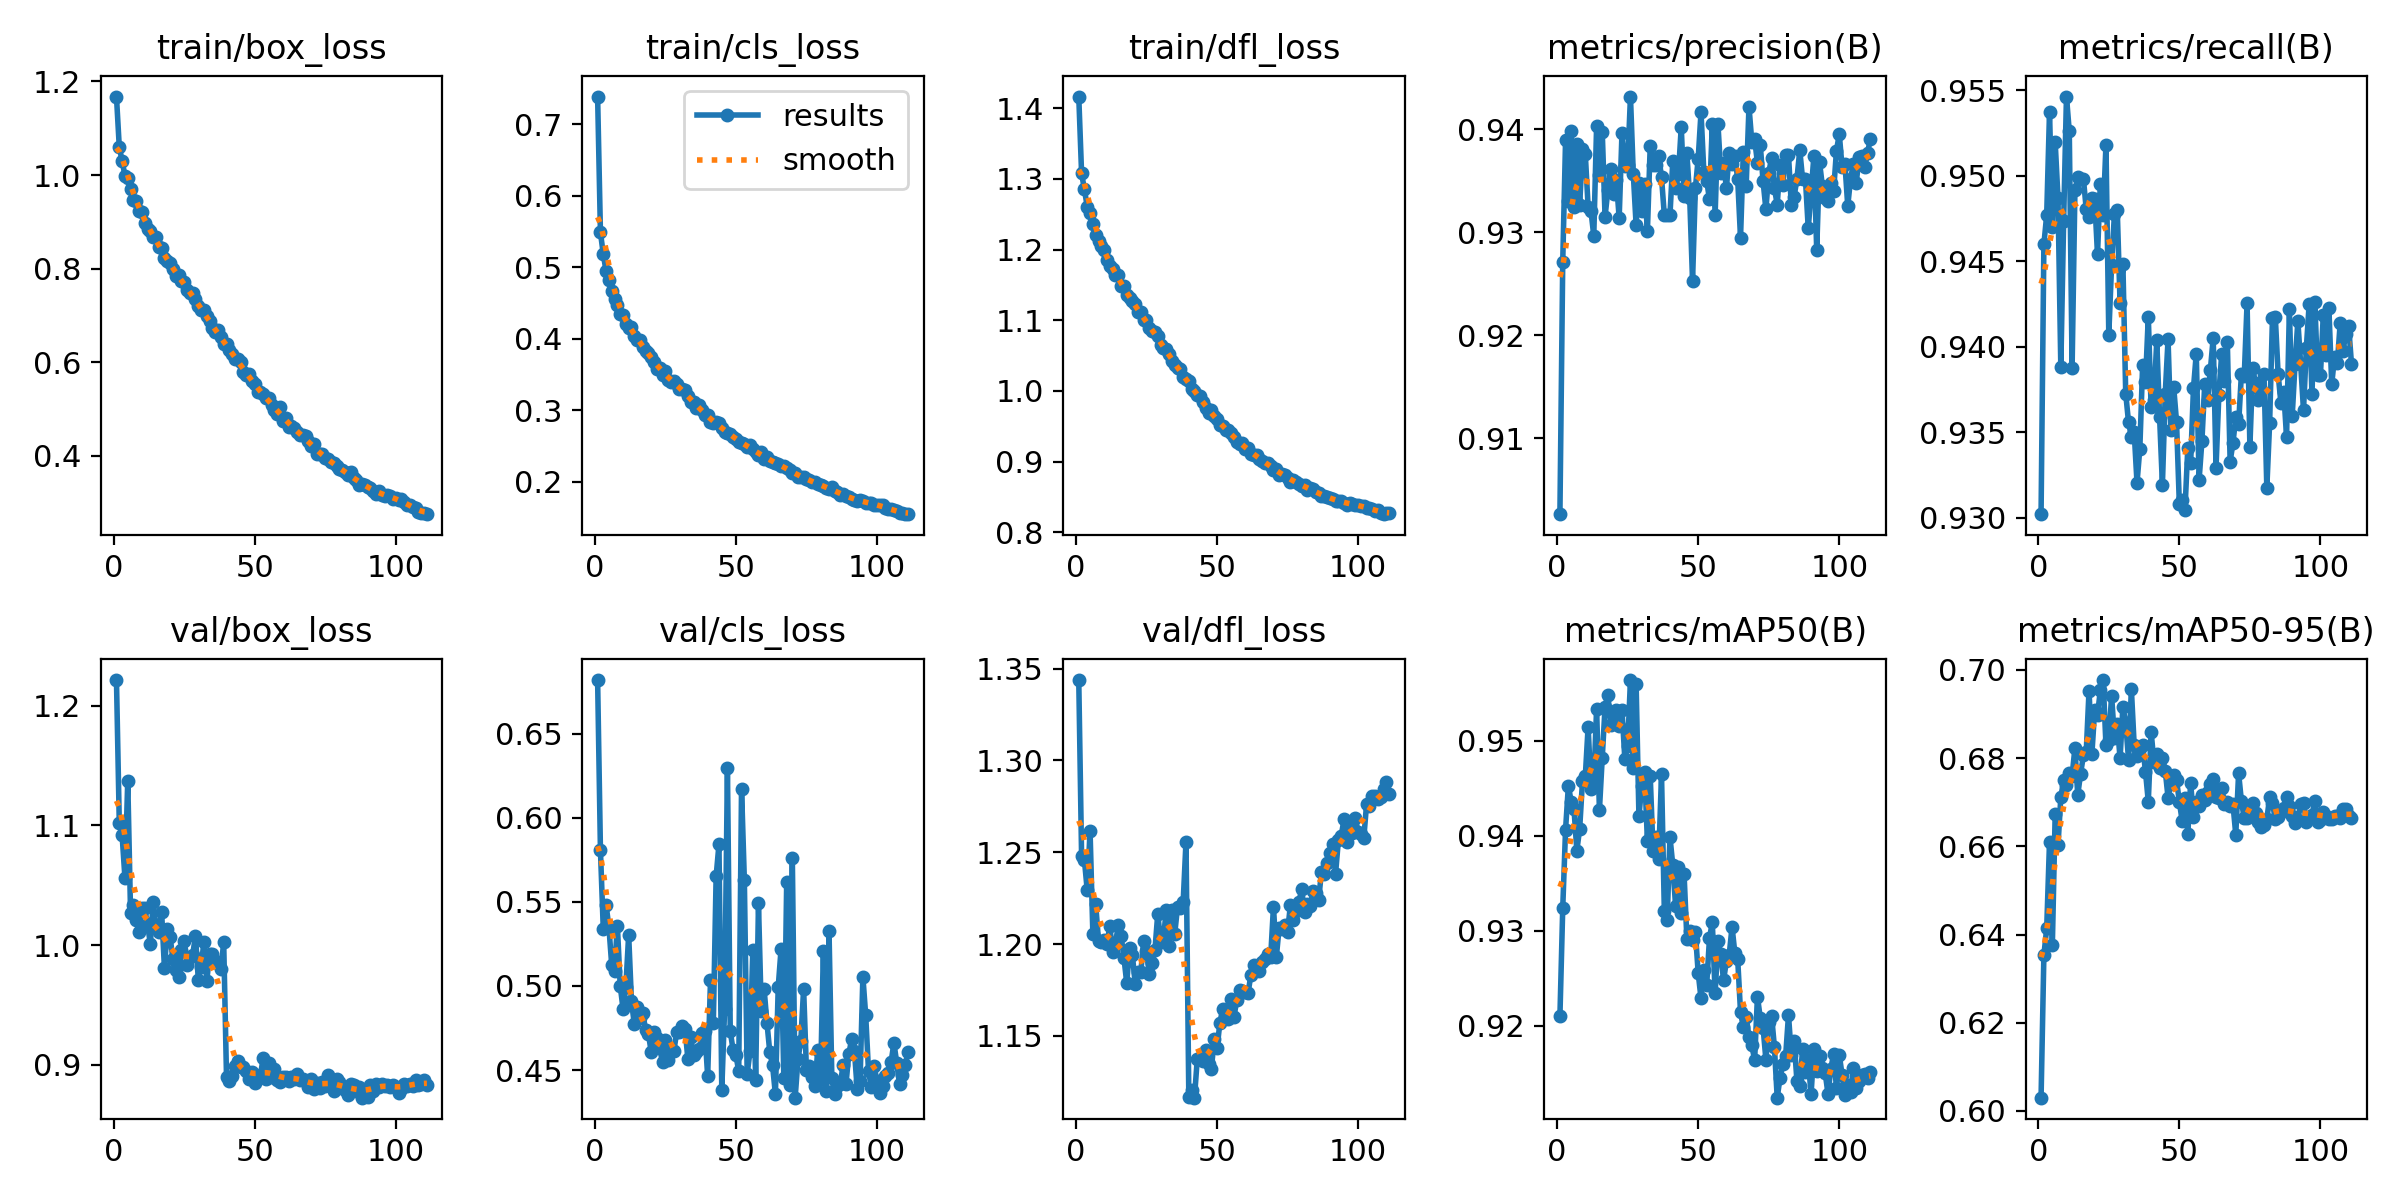
\includegraphics[width=\textwidth]{images/image_ch3/results_recto/results.png}
  \caption{Évolution des pertes et métriques d'entraînement --- CIN Recto}
  \label{fig:ch3-results-recto}
\end{figure}

La Figure~\ref{fig:ch3-results-recto} montre une convergence progressive des pertes d'entraînement et de validation, avec une mAP50 qui atteint 0,953 en fin d'entraînement. Le mAP50-95 global de 0,698 traduit une localisation précise des bounding boxes, ce qui est cohérent avec la complexité du recto --- 10 classes dont plusieurs champs compacts (\texttt{num\_cin}, \texttt{dob}).

\begin{figure}[H]
  \centering
  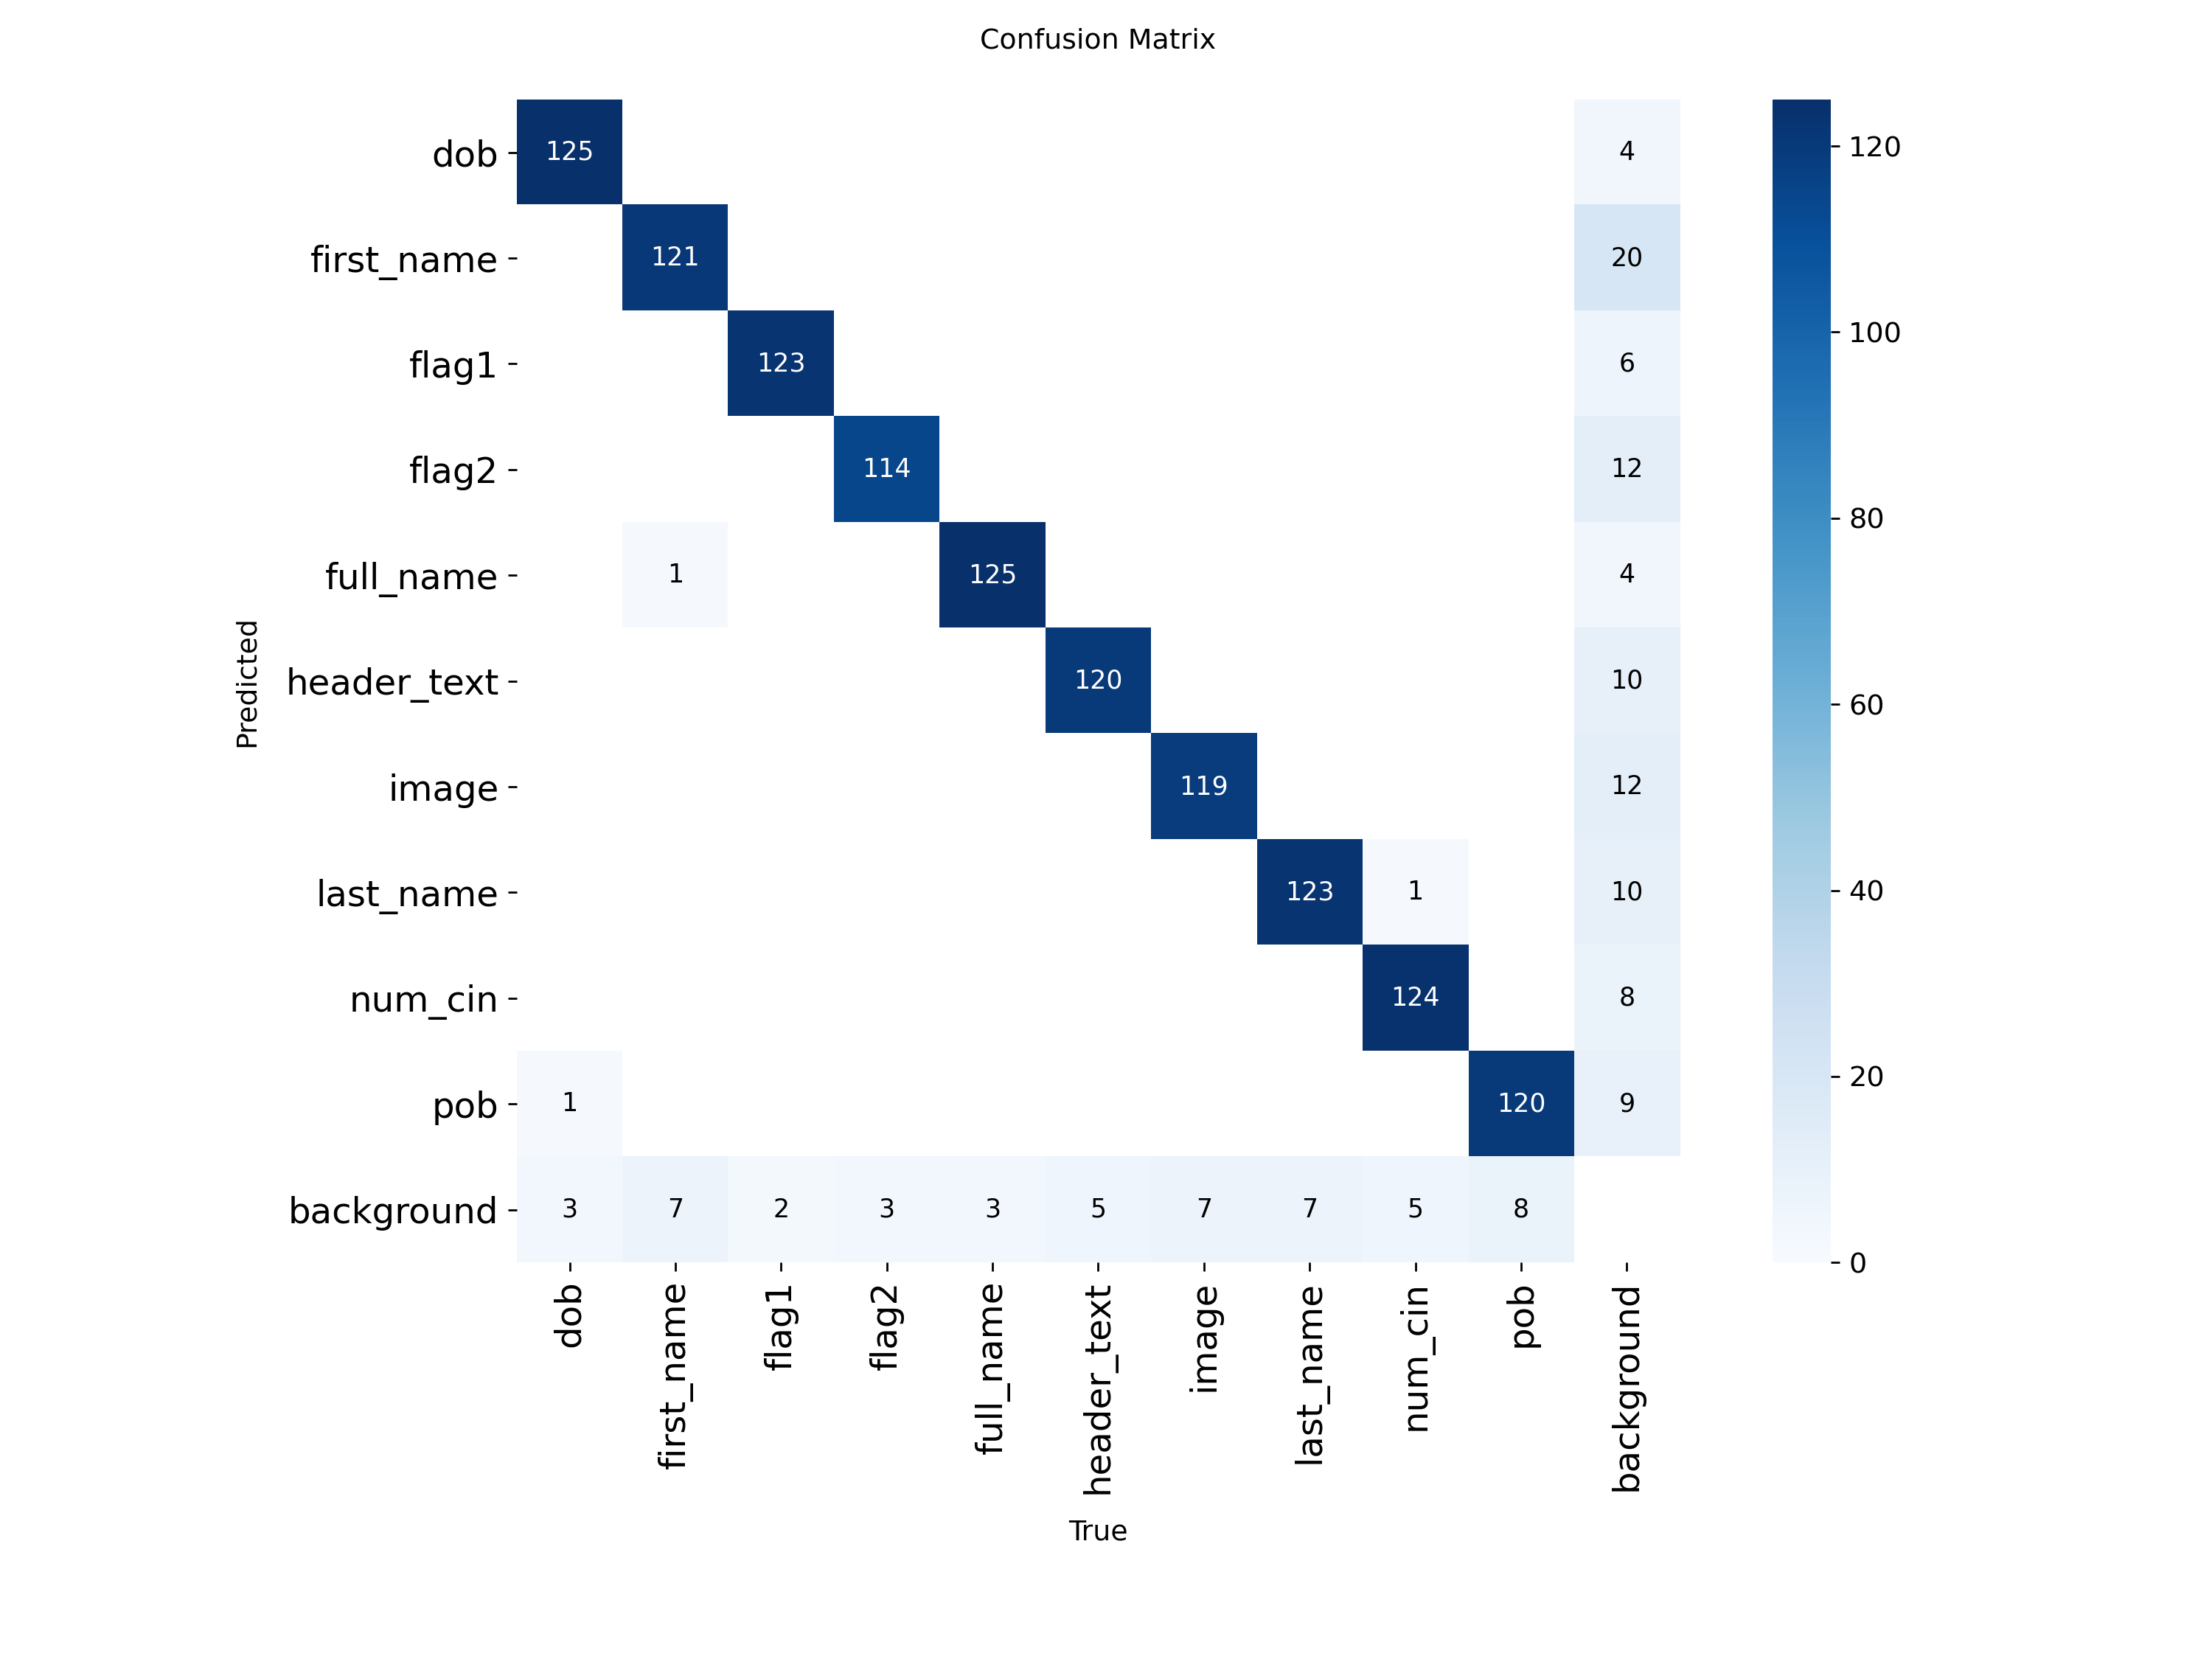
\includegraphics[width=0.80\textwidth]{images/image_ch3/results_recto/confusion_matrix.png}
  \caption{Matrice de confusion --- CIN Recto}
  \label{fig:ch3-cm-recto}
\end{figure}

La matrice de confusion (Figure~\ref{fig:ch3-cm-recto}) confirme la solidité du modèle sur les classes structurées (\texttt{flag1}, \texttt{flag2}, \texttt{num\_cin}). Les confusions les plus notables concernent \texttt{first\_name} et \texttt{pob}, dont la position et la typographie sont proches sur le document.

Le Tableau~\ref{tab:ch3-metrics-recto} présente les métriques détaillées par champ, évaluées sur le jeu de validation (156 images, 1\,267 instances).

\begin{table}[H]
  \centering
  \small
  \begin{tabular}{|l|c|c|c|c|}
    \toprule
    \rowcolor{bleu_principal}
    \textcolor{white}{\textbf{Champ}} & \textcolor{white}{\textbf{Précision}} & \textcolor{white}{\textbf{Rappel}} & \textcolor{white}{\textbf{mAP50}} & \textcolor{white}{\textbf{mAP50-95}} \\
    \midrule
    \texttt{dob}         & 0,973 & 0,969 & 0,963 & 0,649 \\
    \midrule
    \rowcolor{gris_leger}
    \texttt{first\_name} & 0,920 & 0,896 & 0,917 & 0,569 \\
    \midrule
    \texttt{flag1}       & 0,951 & 0,984 & 0,983 & 0,820 \\
    \midrule
    \rowcolor{gris_leger}
    \texttt{flag2}       & 0,924 & 0,940 & 0,976 & 0,815 \\
    \midrule
    \texttt{full\_name}  & 0,961 & 0,971 & 0,970 & 0,645 \\
    \midrule
    \rowcolor{gris_leger}
    \texttt{header\_text}& 0,920 & 0,960 & 0,938 & 0,831 \\
    \midrule
    \texttt{image}       & 0,919 & 0,944 & 0,924 & 0,769 \\
    \midrule
    \rowcolor{gris_leger}
    \texttt{last\_name}  & 0,946 & 0,937 & 0,952 & 0,626 \\
    \midrule
    \texttt{num\_cin}    & 0,956 & 0,954 & 0,969 & 0,667 \\
    \midrule
    \rowcolor{gris_leger}
    \texttt{pob}         & 0,926 & 0,922 & 0,939 & 0,591 \\
    \midrule
    \rowcolor{bleu_clair!15}
    \textbf{Global}      & \textbf{0,940} & \textbf{0,948} & \textbf{0,953} & \textbf{0,698} \\
    \bottomrule
  \end{tabular}
  \caption{Métriques de validation par champ --- modèle CIN Recto}
  \label{tab:ch3-metrics-recto}
\end{table}

\paragraph{CIN Verso}

\begin{figure}[H]
  \centering
  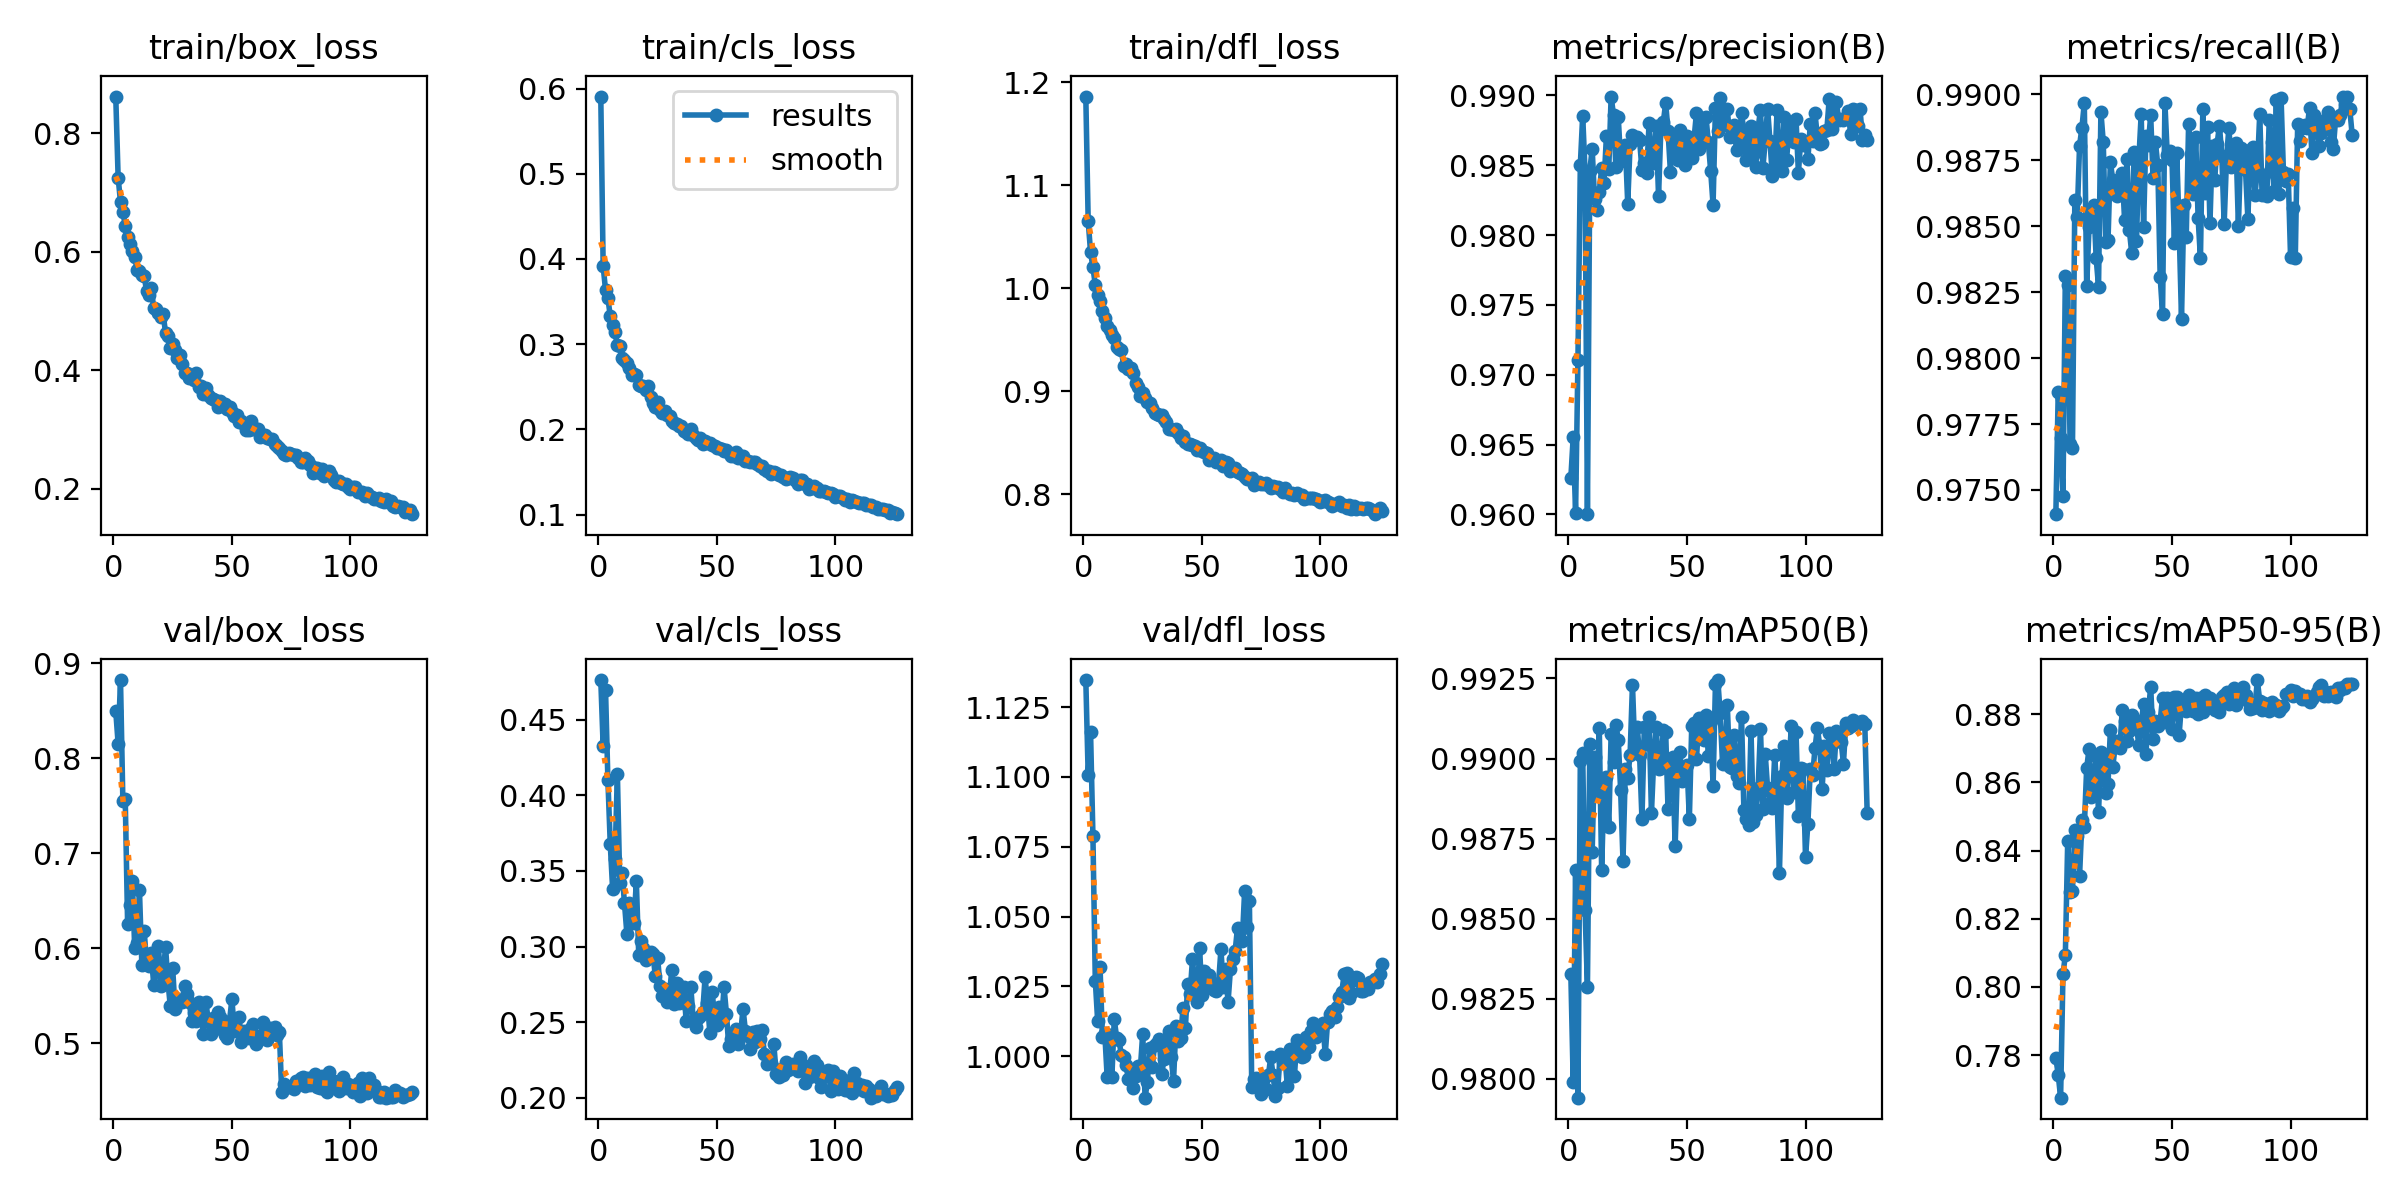
\includegraphics[width=\textwidth]{images/image_ch3/results_verso/results.png}
  \caption{Évolution des pertes et métriques d'entraînement --- CIN Verso}
  \label{fig:ch3-results-verso}
\end{figure}

La Figure~\ref{fig:ch3-results-verso} montre une convergence rapide des trois composantes de perte (box, cls, dfl) dès les 50 premières époques, avec une mAP50 qui se stabilise autour de 0,988 en fin d'entraînement.

\begin{figure}[H]
  \centering
  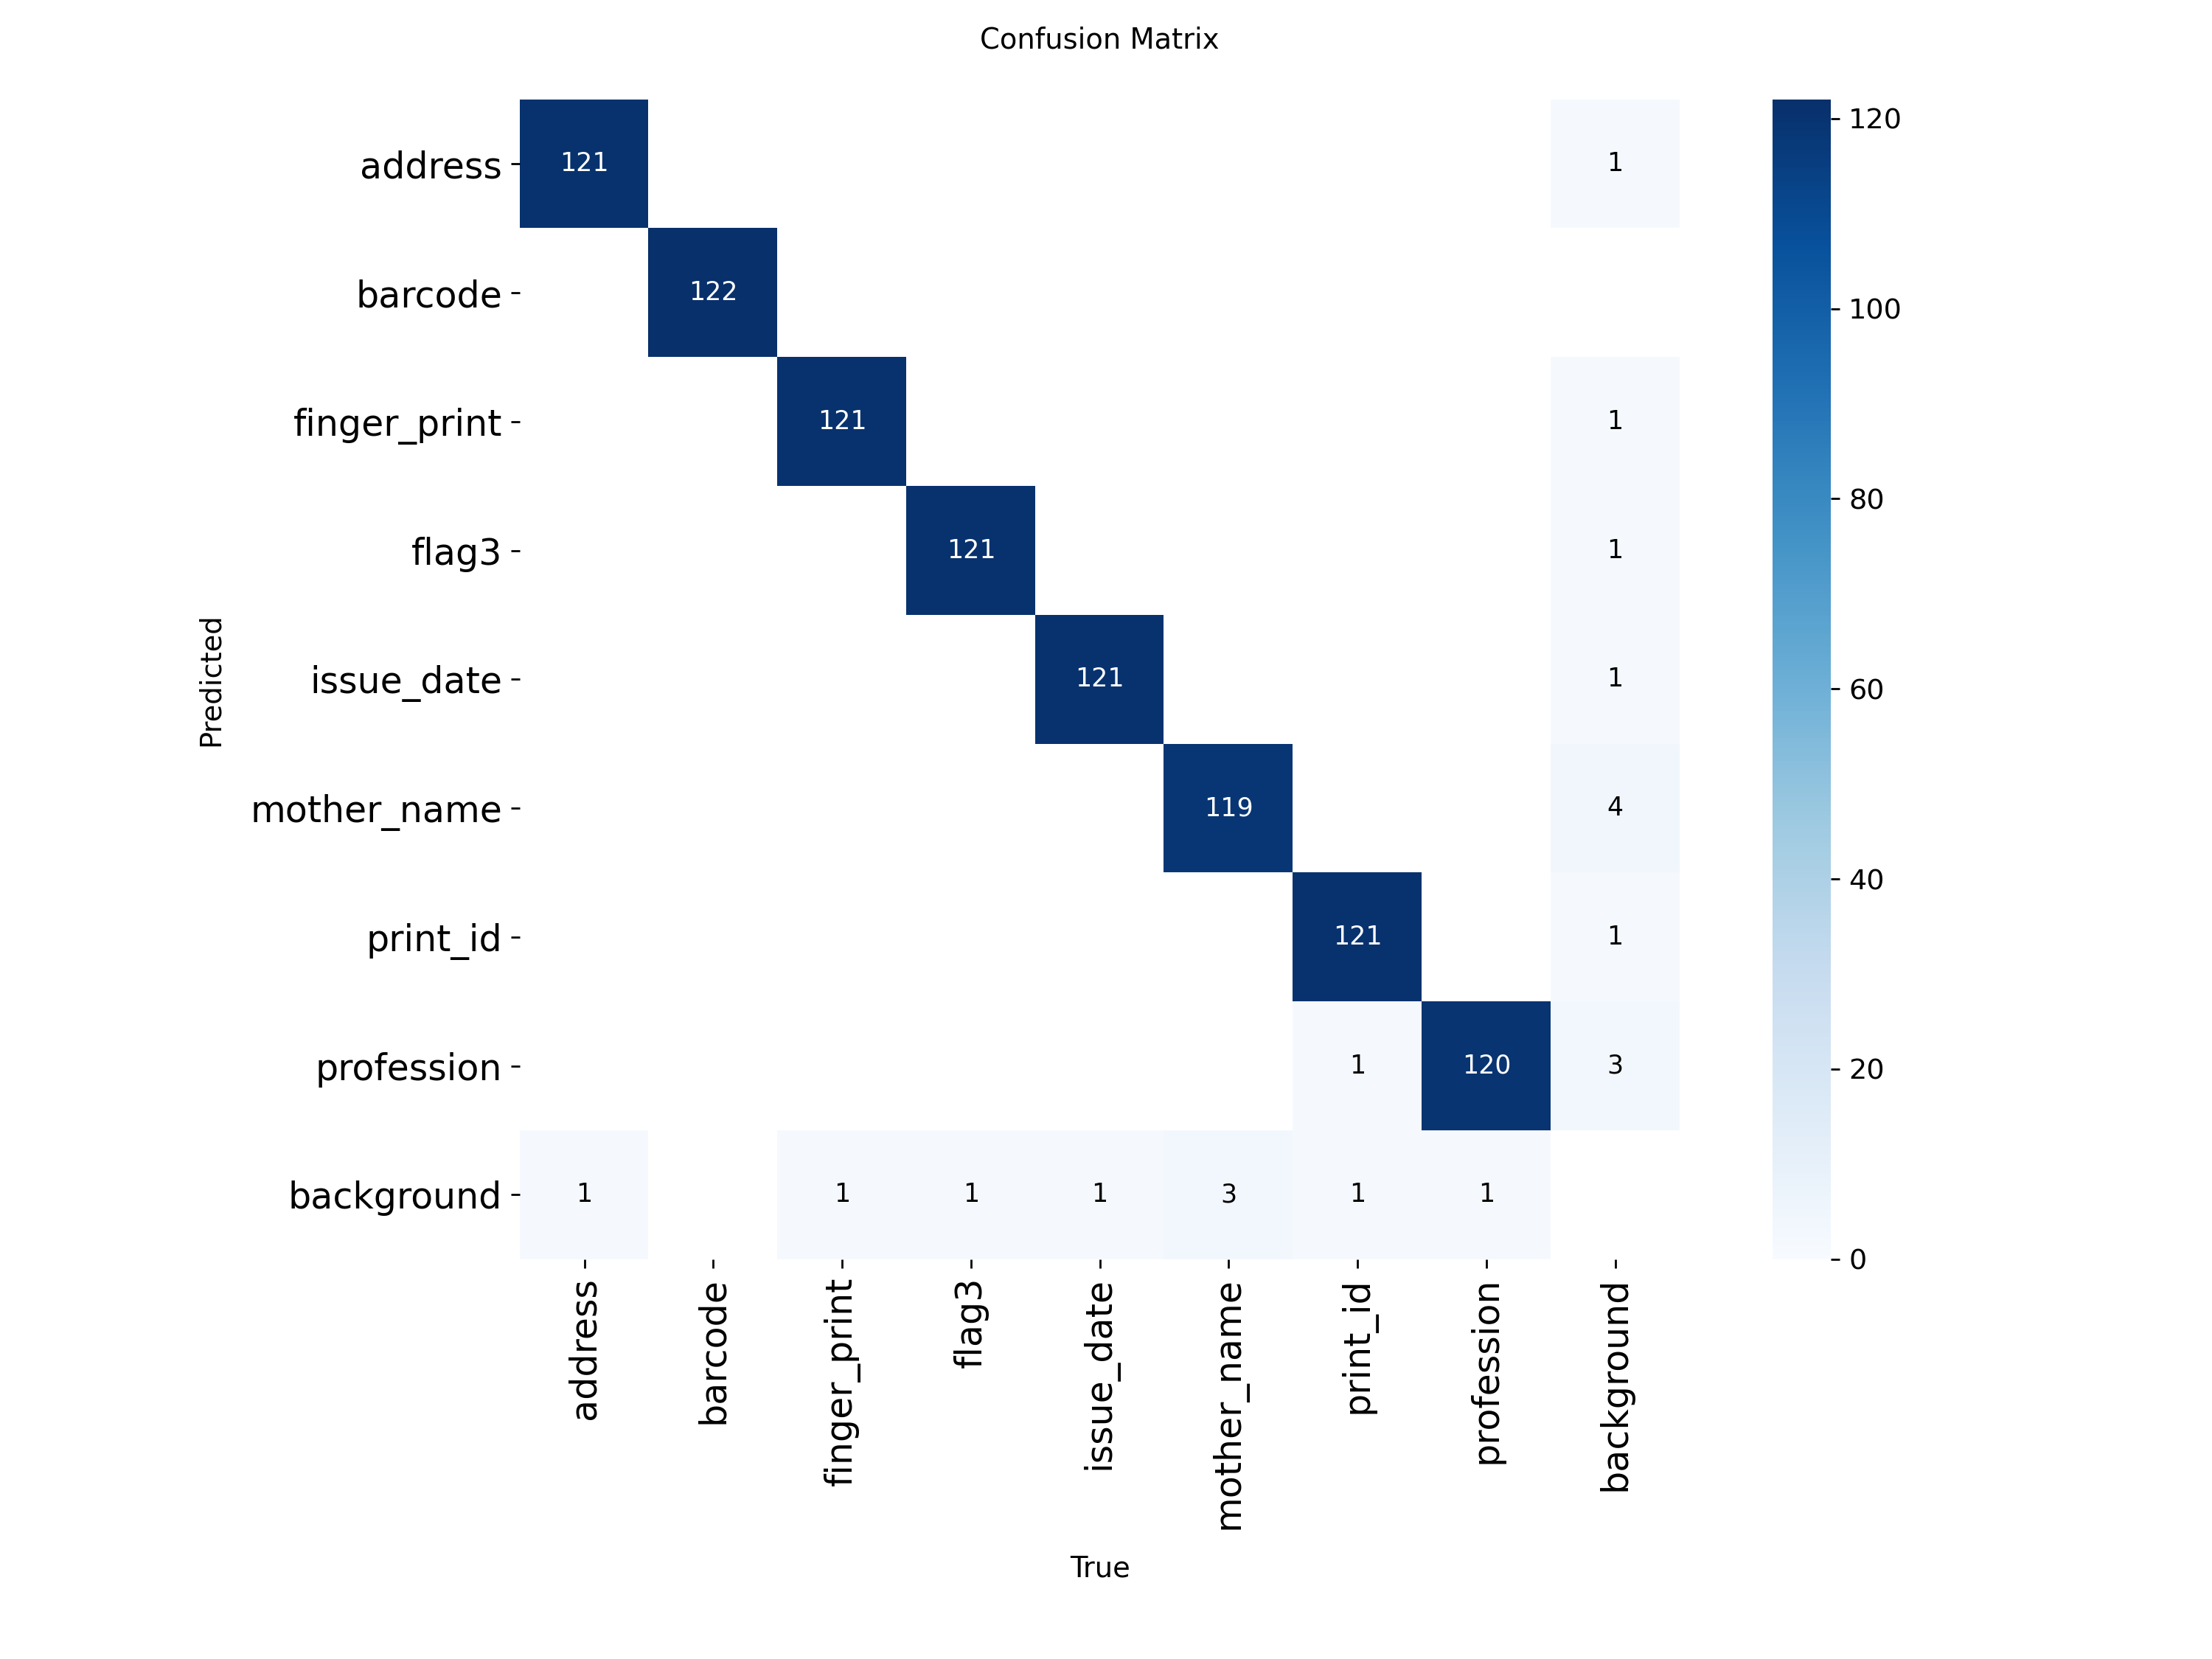
\includegraphics[width=0.80\textwidth]{images/image_ch3/results_verso/confusion_matrix.png}
  \caption{Matrice de confusion --- CIN Verso}
  \label{fig:ch3-cm-verso}
\end{figure}

La matrice de confusion (Figure~\ref{fig:ch3-cm-verso}) révèle que la quasi-totalité des 8 classes sont correctement localisées. Le champ \texttt{mother\_name} présente le plus grand nombre de confusions (4 instances classées en arrière-plan), ce qui s'explique par sa position variable sur le document et la similitude visuelle avec le champ \texttt{profession}.

Le Tableau~\ref{tab:ch3-metrics-verso} présente les métriques détaillées par champ, telles qu'évaluées sur le jeu de validation (148 images, 976 instances).

\begin{table}[H]
  \centering
  \small
  \begin{tabular}{|l|c|c|c|c|}
    \toprule
    \rowcolor{bleu_principal}
    \textcolor{white}{\textbf{Champ}} & \textcolor{white}{\textbf{Précision}} & \textcolor{white}{\textbf{Rappel}} & \textcolor{white}{\textbf{mAP50}} & \textcolor{white}{\textbf{mAP50-95}} \\
    \midrule
    \texttt{address}      & 0,988 & 0,992 & 0,992 & 0,863 \\
    \midrule
    \rowcolor{gris_leger}
    \texttt{barcode}      & 1,000 & 1,000 & 0,995 & 0,969 \\
    \midrule
    \texttt{finger\_print} & 0,988 & 0,992 & 0,994 & 0,976 \\
    \midrule
    \rowcolor{gris_leger}
    \texttt{flag3}        & 0,992 & 0,992 & 0,995 & 0,953 \\
    \midrule
    \texttt{issue\_date}  & 0,992 & 0,990 & 0,994 & 0,928 \\
    \midrule
    \rowcolor{gris_leger}
    \texttt{mother\_name} & 0,952 & 0,959 & 0,961 & 0,792 \\
    \midrule
    \texttt{print\_id}    & 0,987 & 0,984 & 0,984 & 0,903 \\
    \midrule
    \rowcolor{gris_leger}
    \texttt{profession}   & 0,976 & 0,990 & 0,992 & 0,738 \\
    \midrule
    \rowcolor{bleu_clair!15}
    \textbf{Global}       & \textbf{0,984} & \textbf{0,987} & \textbf{0,988} & \textbf{0,890} \\
    \bottomrule
  \end{tabular}
  \caption{Métriques de validation par champ --- modèle CIN Verso}
  \label{tab:ch3-metrics-verso}
\end{table}

\paragraph{Passeport}

\begin{figure}[H]
  \centering
  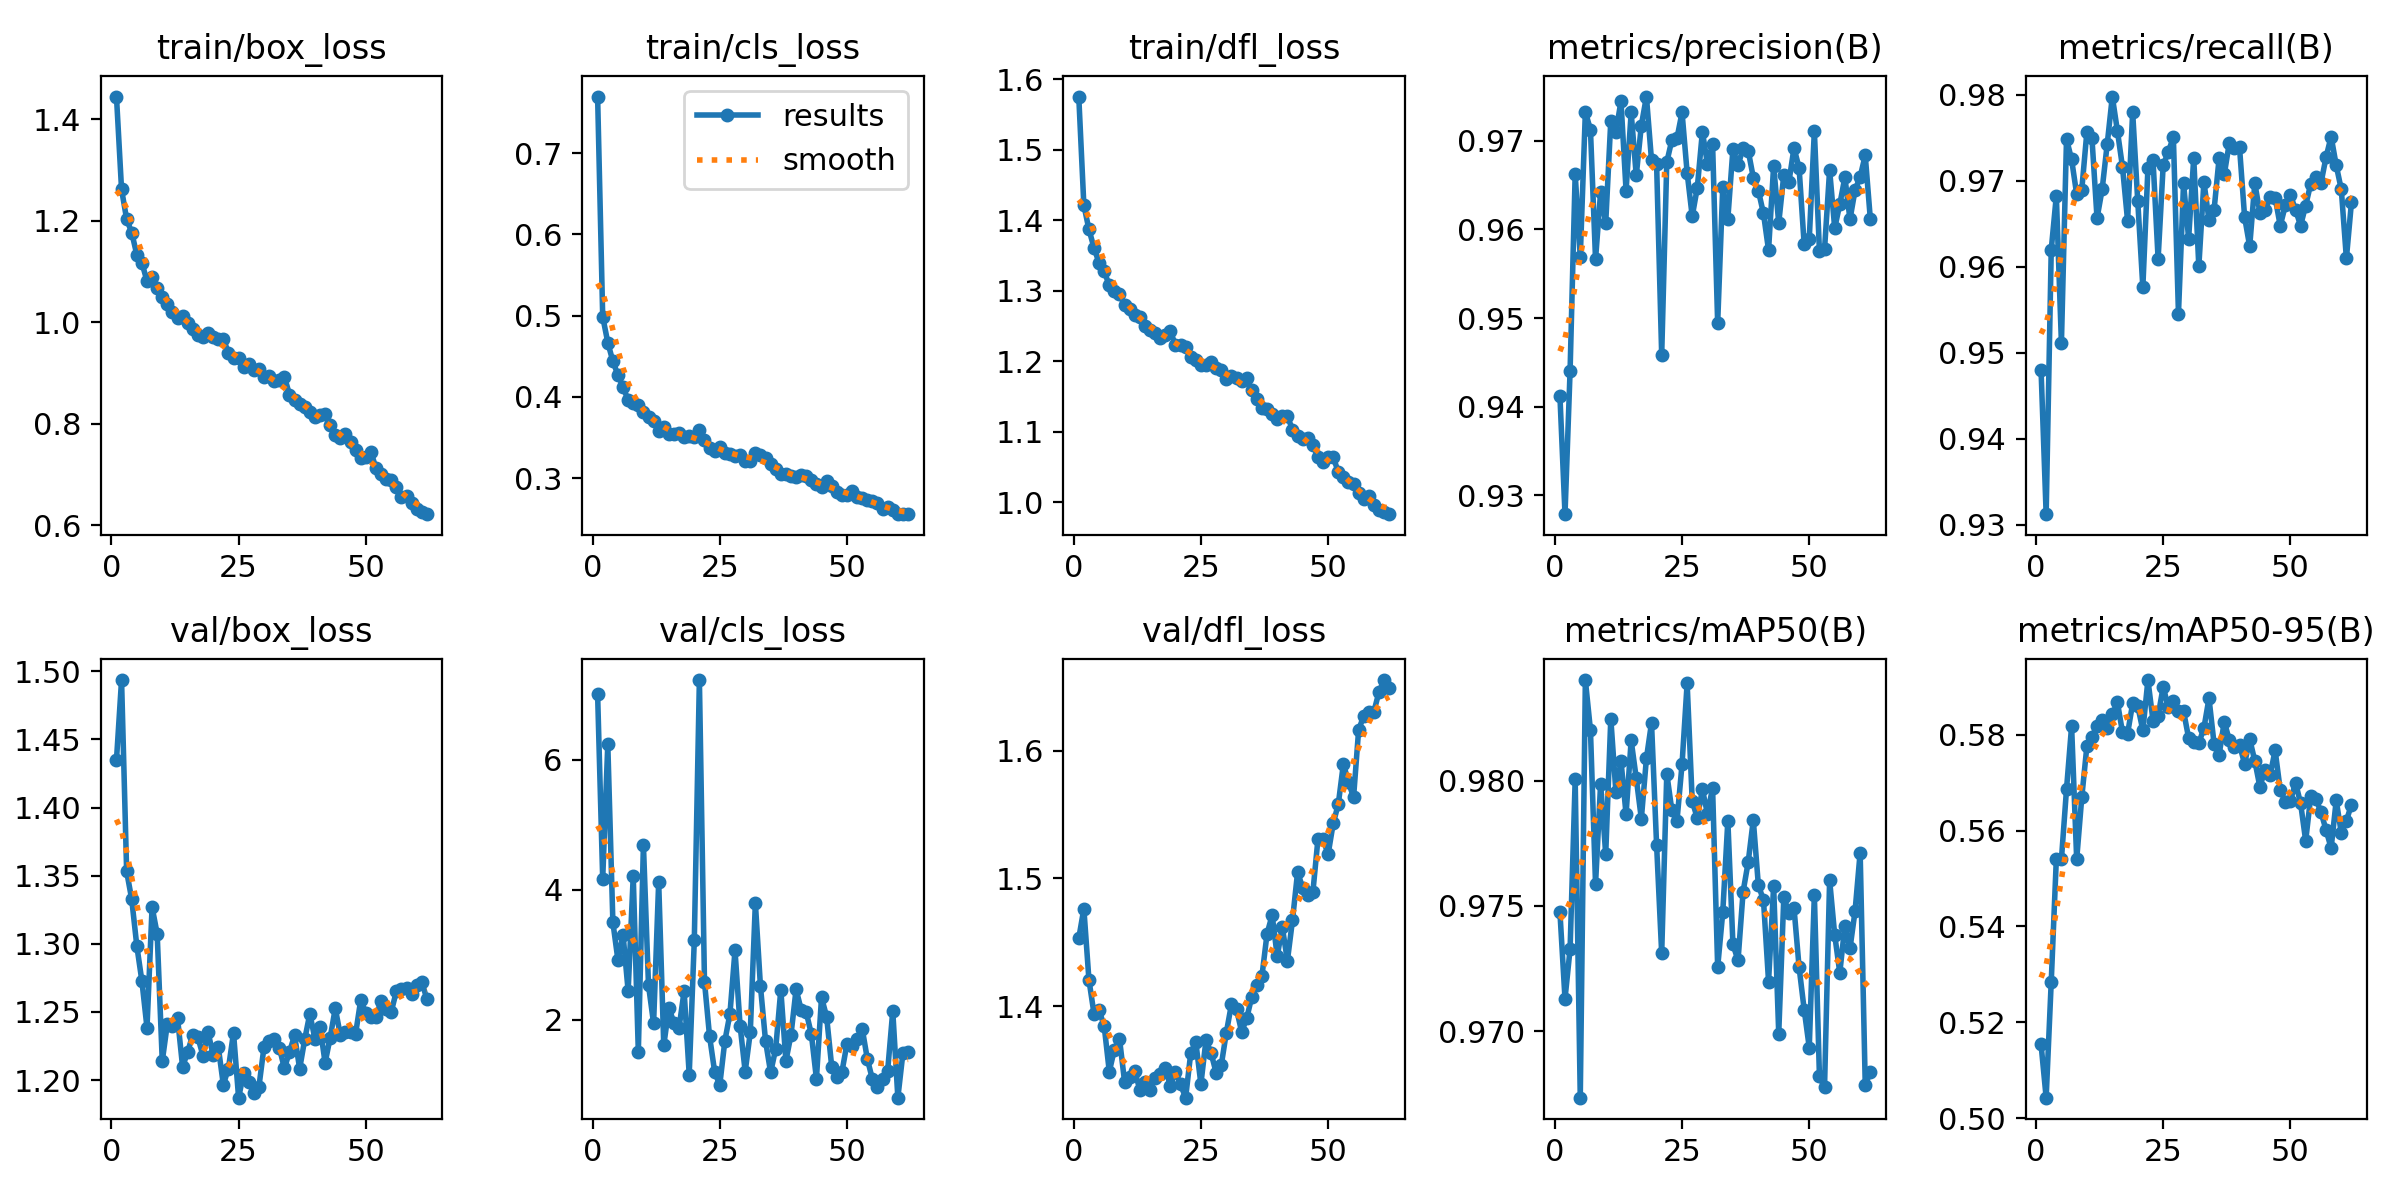
\includegraphics[width=\textwidth]{images/image_ch3/results_passport/results.png}
  \caption{Évolution des pertes et métriques d'entraînement --- Passeport}
  \label{fig:ch3-results-passport}
\end{figure}

La Figure~\ref{fig:ch3-results-passport} illustre une convergence stable, avec une mAP50 finale de 0,980. Le mAP50-95 global de 0,592 est plus bas que pour la CIN, ce qui s'explique par la densité textuelle élevée du passeport (12 classes dont plusieurs champs proches comme \texttt{first\_name}, \texttt{last\_name} et \texttt{full\_name}) et un dataset plus réduit (137 images de validation).

\begin{figure}[H]
  \centering
  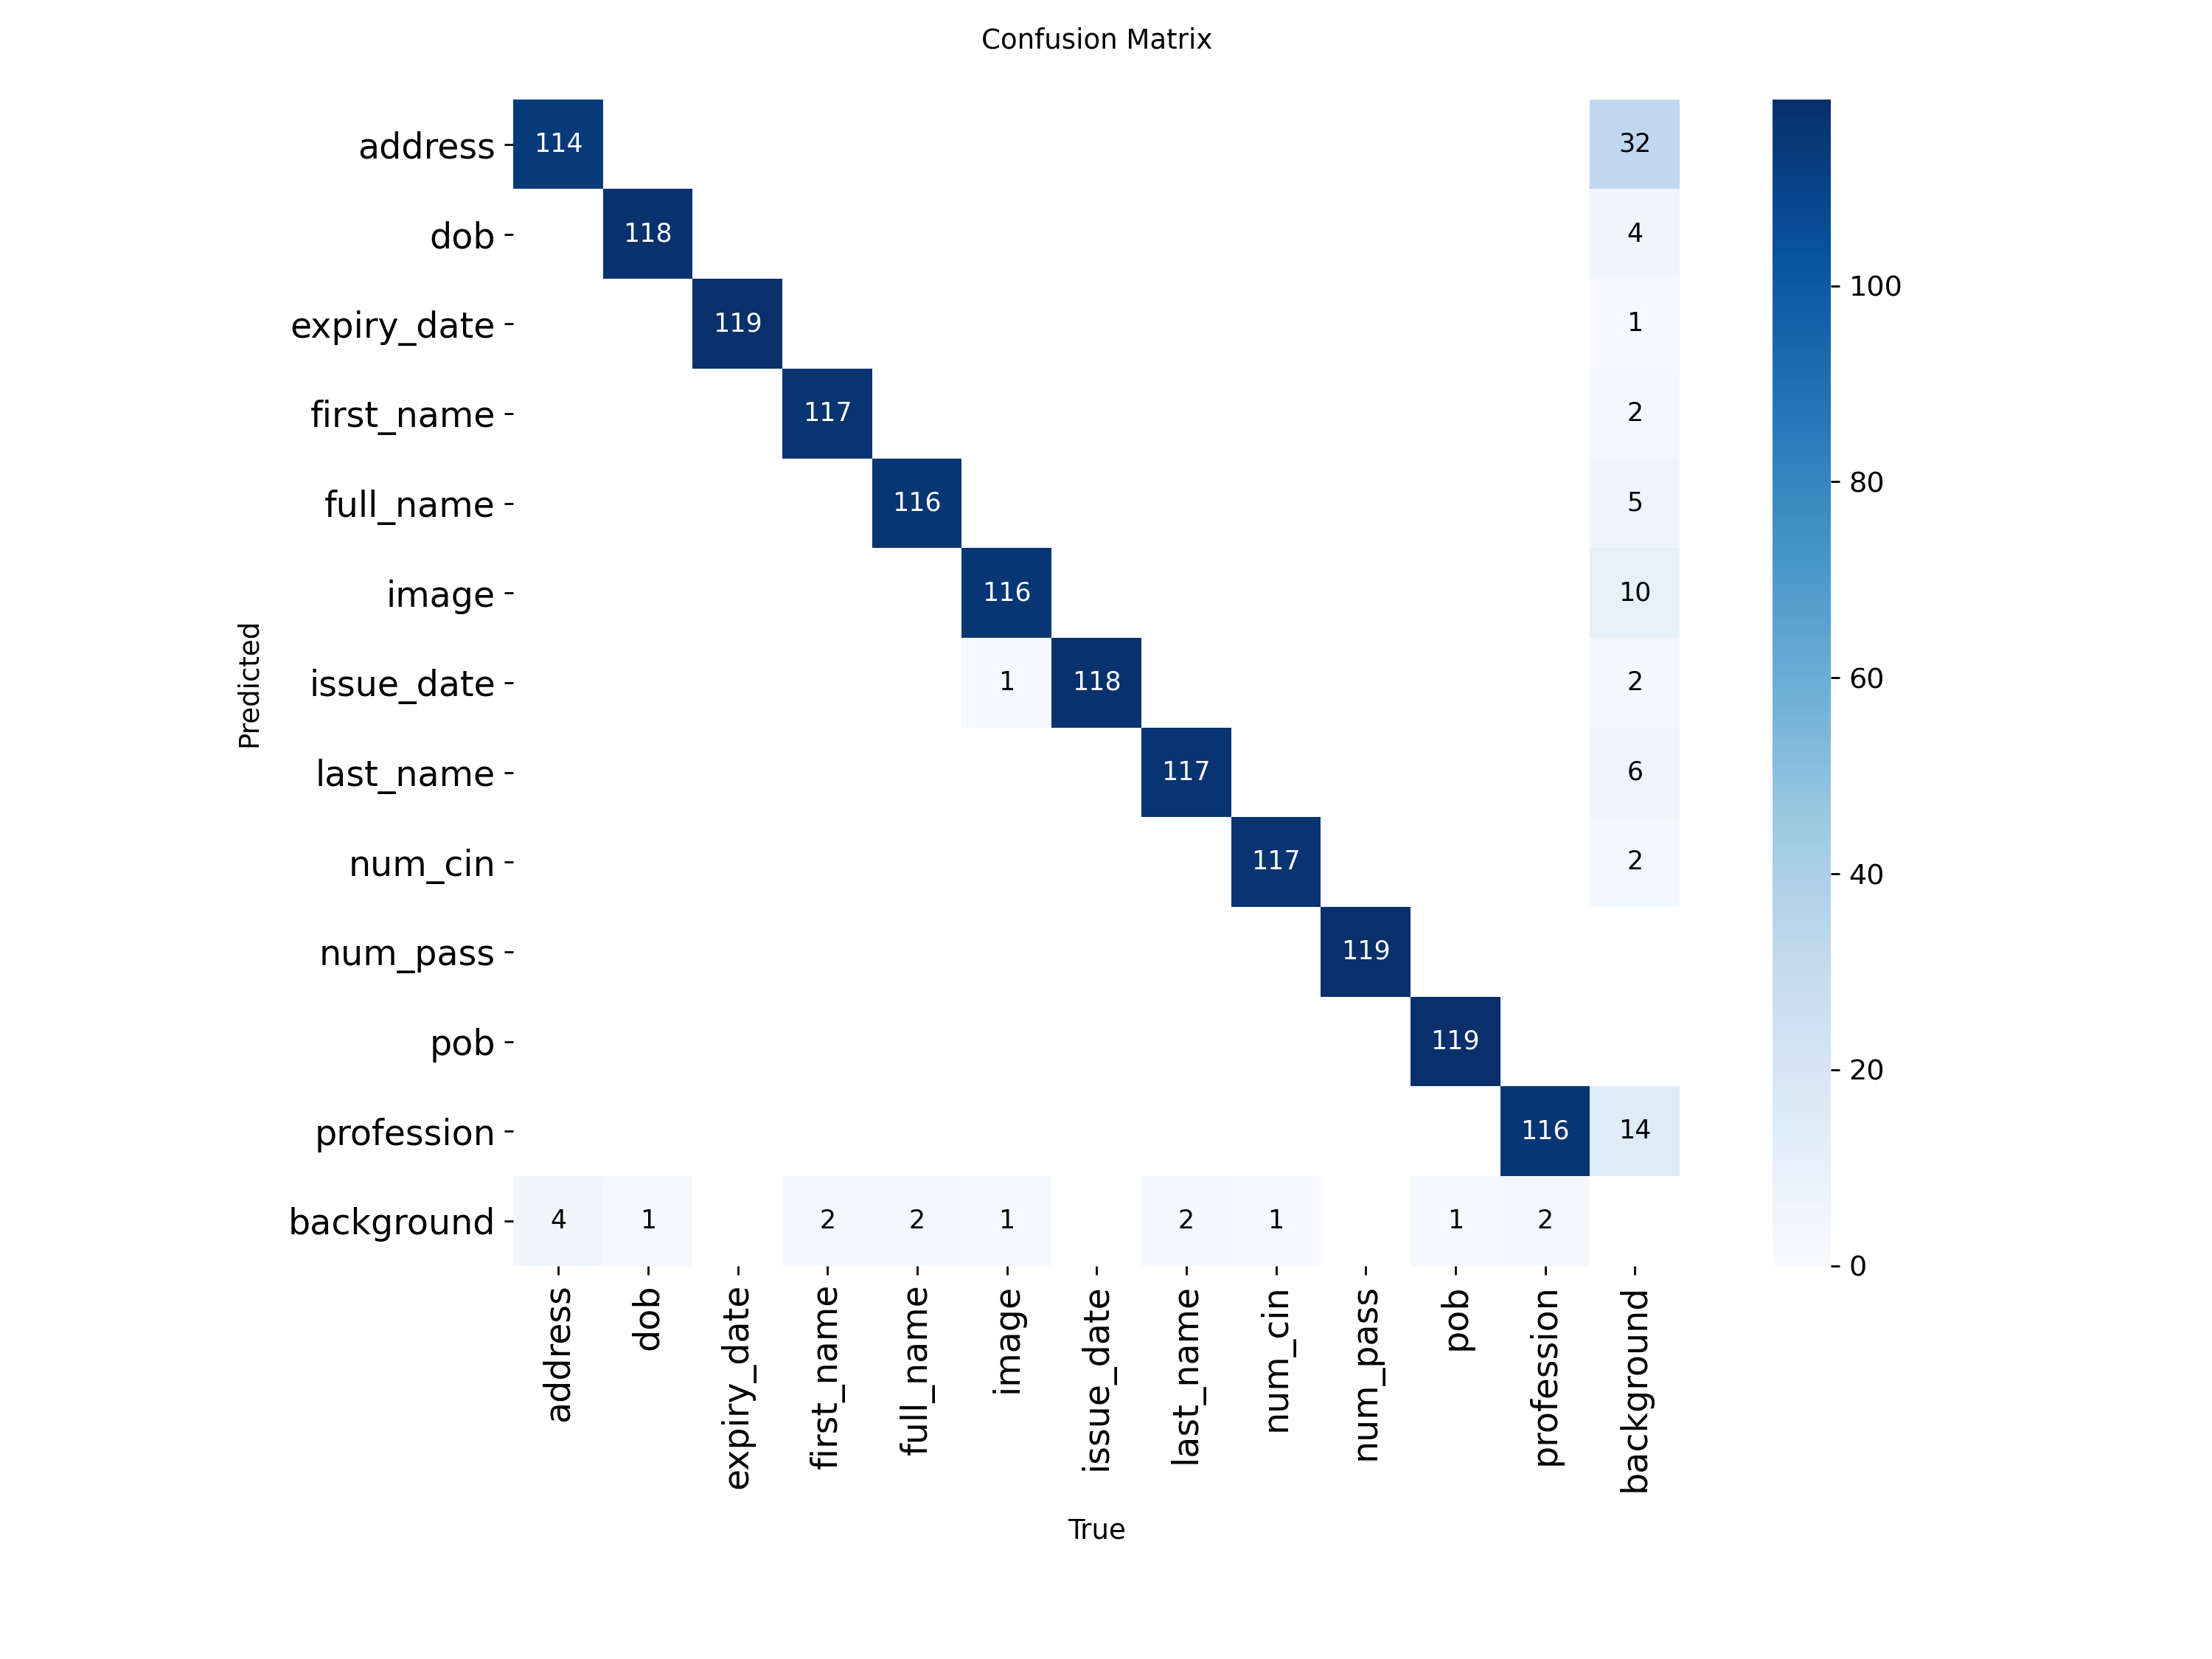
\includegraphics[width=0.80\textwidth]{images/image_ch3/results_passport/confusion_matrix.png}
  \caption{Matrice de confusion --- Passeport}
  \label{fig:ch3-cm-passport}
\end{figure}

La matrice de confusion (Figure~\ref{fig:ch3-cm-passport}) confirme d'excellentes performances sur les champs structurés (\texttt{num\_pass}, \texttt{pob}, \texttt{image}). Le champ \texttt{address} présente le rappel le plus bas (0,856), attribuable à sa position variable selon les versions du passeport tunisien.

Le Tableau~\ref{tab:ch3-metrics-passport} présente les métriques détaillées par champ, évaluées sur le jeu de validation (137 images, 1\,423 instances).

\begin{table}[H]
  \centering
  \small
  \begin{tabular}{|l|c|c|c|c|}
    \toprule
    \rowcolor{bleu_principal}
    \textcolor{white}{\textbf{Champ}} & \textcolor{white}{\textbf{Précision}} & \textcolor{white}{\textbf{Rappel}} & \textcolor{white}{\textbf{mAP50}} & \textcolor{white}{\textbf{mAP50-95}} \\
    \midrule
    \texttt{address}     & 0,936 & 0,856 & 0,950 & 0,540 \\
    \midrule
    \rowcolor{gris_leger}
    \texttt{dob}         & 0,963 & 0,975 & 0,982 & 0,599 \\
    \midrule
    \texttt{expiry\_date}& 0,992 & 0,995 & 0,995 & 0,583 \\
    \midrule
    \rowcolor{gris_leger}
    \texttt{first\_name} & 0,974 & 0,963 & 0,950 & 0,512 \\
    \midrule
    \texttt{full\_name}  & 0,976 & 0,975 & 0,989 & 0,664 \\
    \midrule
    \rowcolor{gris_leger}
    \texttt{image}       & 0,943 & 0,988 & 0,992 & 0,840 \\
    \midrule
    \texttt{issue\_date} & 0,975 & 0,983 & 0,971 & 0,565 \\
    \midrule
    \rowcolor{gris_leger}
    \texttt{last\_name}  & 0,958 & 0,983 & 0,976 & 0,569 \\
    \midrule
    \texttt{num\_cin}    & 0,983 & 0,992 & 0,992 & 0,572 \\
    \midrule
    \rowcolor{gris_leger}
    \texttt{num\_pass}   & 0,999 & 1,000 & 0,995 & 0,544 \\
    \midrule
    \texttt{pob}         & 0,997 & 0,992 & 0,995 & 0,609 \\
    \midrule
    \rowcolor{gris_leger}
    \texttt{profession}  & 0,923 & 0,958 & 0,979 & 0,501 \\
    \midrule
    \rowcolor{bleu_clair!15}
    \textbf{Global}      & \textbf{0,968} & \textbf{0,971} & \textbf{0,980} & \textbf{0,592} \\
    \bottomrule
  \end{tabular}
  \caption{Métriques de validation par champ --- modèle Passeport}
  \label{tab:ch3-metrics-passport}
\end{table}

%-------------------------------------------------------------
\subsection{Extraction texte --- PaddleOCR PP-OCRv5}
\label{subsec:paddleocr-extraction}
%-------------------------------------------------------------

Comme présenté au chapitre 2, PP-OCRv5 a été retenu pour ses performances sur les scripts arabes et latins simultanément, sa légèreté et sa compatibilité avec un déploiement \textit{on-premise}. Dans le pipeline, il reçoit en entrée les crops produits par YOLOv11m et retourne le texte structuré de chaque champ.

\subsubsection*{Workflow d'extraction}

Le pipeline d'extraction suit quatre étapes enchaînées pour chaque zone détectée par YOLO :

\begin{enumerate}
  \item \textbf{Recadrage (crop)} : la bounding box YOLO est appliquée à l'image haute résolution. Des ajustements fins compensent les légères sous-détections :
  \begin{itemize}
    \item Élargissement des bords pour les dates du passeport.
    \item Réduction à droite pour l'adresse verso (exclure le label « العنوان » imprimé).
    \item Conservation des trois quarts supérieurs pour le champ nom recto.
  \end{itemize}

  \item \textbf{Prétraitement (preprocessing)} : plusieurs traitements sont appliqués selon la qualité du crop :
  \begin{itemize}
    \item Ajout d'une bordure blanche de 40 pixels sur chaque côté.
    \item Si hauteur $<$ 80 px : agrandissement par interpolation Lanczos4.
    \item Pour les champs sur fond texturé : binarisation adaptative pour séparer texte et fond.
  \end{itemize}

  \item \textbf{Lecture OCR} : deux moteurs fonctionnent en parallèle selon la langue du champ :
  \begin{itemize}
    \item Moteur arabe : champs identitaires (nom, prénom, adresse).
    \item Moteur latin : champs numériques et dates.
    \item Si score moyen $<$ 0,5 : second passage automatique sur image binarisée.
  \end{itemize}

  \item \textbf{Post-traitement} : normalisation, correction et structuration du texte brut en JSON (détaillé ci-après).
\end{enumerate}

\subsubsection*{Prétraitement : gestion des petits crops}

La résolution des crops varie fortement selon la taille du champ sur le document original. Un champ \texttt{num\_cin} (8 chiffres) occupe typiquement 60 à 70 pixels de hauteur après recadrage — en dessous du seuil de lisibilité optimal de PaddleOCR. Le Tableau~\ref{tab:ch3-preprocessing} synthétise les quatre problèmes identifiés et les solutions appliquées.

\begin{table}[H]
  \centering
  \small
  \begin{tabular}{|p{4cm}|p{4cm}|p{5cm}|}
    \toprule
    \rowcolor{bleu_principal}
    \textcolor{white}{\textbf{Problème}} & \textcolor{white}{\textbf{Solution}} & \textcolor{white}{\textbf{Paramètre}} \\
    \midrule
    Texte trop petit ($<$ 80 px hauteur) & Agrandissement & Lanczos4, jusqu'à 80 px min \\
    \midrule
    \rowcolor{gris_leger}
    Bords coupés par YOLO & Bordure blanche & 40 px sur chaque côté \\
    \midrule
    Fond texturé (filigrane) & Binarisation adaptative & Seuil automatique \\
    \midrule
    \rowcolor{gris_leger}
    Score OCR faible ($<$ 0,5) & Second passage & Image binarisée en fallback \\
    \bottomrule
  \end{tabular}
  \caption{Traitements de prétraitement appliqués aux crops YOLO}
  \label{tab:ch3-preprocessing}
\end{table}

\subsubsection*{Post-traitement et structuration JSON}

% ── Bloc OCR ─────────────────────────────────────────────────


\medskip
\noindent Le Tableau~\ref{tab:ch3-json-sortie} illustre la structure JSON finale générée pour une CIN, telle qu'observée dans les fichiers de test réels du projet.

\begin{table}[H]
  \centering
  \small
  \begin{tabular}{|l|l|c|}
    \toprule
    \rowcolor{bleu_principal}
    \textcolor{white}{\textbf{Champ JSON}} & \textcolor{white}{\textbf{Exemple de valeur}} & \textcolor{white}{\textbf{Score OCR}} \\
    \midrule
    \texttt{cin\_number} & \texttt{00696358} & 0,9999 \\
    \midrule
    \rowcolor{gris_leger}
    \texttt{nom} & \texttt{الطياري} & 0,9351 \\
    \midrule
    \texttt{prenom} & \texttt{المنجي} & 0,9958 \\
    \midrule
    \rowcolor{gris_leger}
    \texttt{nom\_complet} & \texttt{بن الجيلاني بن محمد} & 0,9528 \\
    \midrule
    \texttt{date\_naissance} & \texttt{19562 سبتمبر} & 0,8746 \\
    \midrule
    \rowcolor{gris_leger}
    \texttt{lieu\_naissance} & \texttt{منوبة} & 0,9954 \\
    \midrule
    \texttt{nom\_mere} & \texttt{الما جري نور} & 0,8840 \\
    \midrule
    \rowcolor{gris_leger}
    \texttt{profession} & \texttt{مستشار قانوني} & 0,8915 \\
    \midrule
    \texttt{adresse} & \texttt{نهج الاستقلال العمران} & 0,8794 \\
    \midrule
    \rowcolor{gris_leger}
    \texttt{issue\_date} & \texttt{2022 سبتمبر} & 0,9423 \\
    \midrule
    \texttt{print\_id} & \texttt{01815766} & 1,0000 \\
    \midrule
    \rowcolor{gris_leger}
    \textbf{Score global} & & \textbf{0,922} \\
    \bottomrule
  \end{tabular}
  \caption{Exemple de sortie JSON structurée --- CIN (extrait réel du projet)}
  \label{tab:ch3-json-sortie}
\end{table}

%-------------------------------------------------------------
\subsection{Configuration matérielle et environnement}
\label{subsec:config-materielle}
%-------------------------------------------------------------

L'ensemble des entraînements a été réalisé sur Google Colab Pro avec un GPU NVIDIA Tesla T4 (16 Go VRAM), en utilisant le framework Ultralytics dans sa version compatible YOLOv11. Le Tableau~\ref{tab:ch3-config-materielle} résume la configuration complète.

\small
\begin{longtable}{|l|l|}
  \rowcolor{bleu_principal}
  \textcolor{white}{\textbf{Composant}} & \textcolor{white}{\textbf{Valeur}} \\
  \endfirsthead
  \rowcolor{bleu_principal}
  \textcolor{white}{\textbf{Composant}} & \textcolor{white}{\textbf{Valeur}} \\
  \endhead
  \midrule
  GPU (entraînement) & NVIDIA Tesla T4 --- 16 Go VRAM \\
  \midrule
  \rowcolor{gris_leger}
  Environnement & Google Colab Pro \\
  \midrule
  Framework détection & Ultralytics (YOLOv11m) \\
  \midrule
  \rowcolor{gris_leger}
  Framework OCR & PaddleOCR PP-OCRv5 \\
  \midrule
  Langage & Python 3.11 \\
  \midrule
  \rowcolor{gris_leger}
  Gestionnaire de dataset & Roboflow \\
  \midrule
  Stockage objets & MinIO (déploiement \textit{on-premise}) \\
  \midrule
  \rowcolor{gris_leger}
  Batch size & 8 (limité par la VRAM à 1280 px) \\
  \midrule
  Résolution d'inférence (OCR) & 1280 $\times$ 1280 px \\
  \midrule
  \rowcolor{gris_leger}
  Résolution d'inférence (capture) & 640 $\times$ 640 px \\
  \midrule
  Temps d'entraînement CIN Recto & \textnormal{[À COMPLÉTER]} \\
  \midrule
  \rowcolor{gris_leger}
  Temps d'entraînement CIN Verso & \textnormal{[À COMPLÉTER]} \\
  \midrule
  Temps d'entraînement Passeport & \textnormal{[À COMPLÉTER]} \\
  \bottomrule
  \caption{Configuration matérielle et environnement d'entraînement}
  \label{tab:ch3-config-materielle}
\end{longtable}
\normalsize


%=============================================================
\section{Évaluation et assurance qualité}
\label{sec:evaluation-qualite}
%=============================================================

Cette section présentera les métriques d'évaluation retenues (mAP, Precision, Recall) sur le jeu de test, ainsi que les résultats des tests de robustesse conduits sur des cas bruités et complexes.

À compléter.


%=============================================================
\section{Déploiement et intégration}
\label{sec:deploiement-integration}
%=============================================================

Cette section décrira l'intégration du pipeline IA dans le backend de l'application via une API FastAPI, en précisant les endpoints exposés, les formats d'échange et les contraintes de performance en production.

À compléter.


%=============================================================
\section{Surveillance et maintenance}
\label{sec:surveillance-maintenance}
%=============================================================

Cette section abordera la stratégie de surveillance du modèle en production, notamment la détection de la dérive des données (\textit{model drift}) en cas d'évolution des formats de documents, ainsi que le protocole de ré-entraînement prévu.

À compléter.


\section*{Conclusion du chapitre}

Ce chapitre a présenté la mise en œuvre complète du premier incrément IA selon la méthodologie CRISP-ML(Q). La phase d'ingénierie des données --- collecte hybride, restauration par Deep Inpainting, génération automatisée, labellisation rigoureuse et augmentation contrôlée --- a fourni la base d'apprentissage. La phase de modélisation a décrit les trois modèles YOLOv11m spécialisés et le pipeline d'extraction OCR complet, depuis le recadrage jusqu'à la structuration JSON finale, avec les paramètres réels d'entraînement et les exemples de sorties du projet. Les sections d'évaluation, de déploiement et de surveillance complèteront ce cycle lors des prochaines étapes du projet.
